%\usepackage{scicite}
%\usepackage{times}
%\usepackage{graphicx}
%\usepackage{verbatim}
%\usepackage{subfigure}
%\usepackage{tikz}
%\usepackage{array}
%\usepackage{tabularx}
%\usepackage{multirow}
%\usepackage{multicol}
%\usepackage{multibox}
%\usepackage{rotating}
%\usepackage{layout}
%\usepackage{epstopdf}
%\usepackage{afterpage}
%\usepackage[left]{lineno}

%% PNAStmpl.tex
%% Template file to use for PNAS articles prepared in LaTeX
%% Version: Apr 14, 2008

%%%%%%%%%%%%%%%%%%%%%%%%%%%%%%
%% BASIC CLASS FILE

\documentclass{pnastwo}

%%%%%%%%%%%%%%%%%%%%%%%%%%%%%%
%% OPTIONAL GRAPHICS STYLE FILE

\usepackage[pdftex]{graphicx}

%%%%%%%%%%%%%%%%%%%%%%%%%%%%%%
%% OPTIONAL POSTSCRIPT FONT FILES

\usepackage{pnastwoF}

%%%%%%%%%%%%%%%%%%%%%%%%%%%%%%
%% ADDITIONAL OPTIONAL STYLE FILES

%\usepackage{amssymb,amsfonts,amsmath}
\usepackage{amsmath}
\usepackage{amssymb}

\usepackage[font=large]{caption}
\usepackage{subfigure}
\usepackage{epstopdf}
\usepackage{graphicx}
\usepackage{verbatim}
\usepackage{array}
\usepackage{tabularx}
\usepackage{multirow}
\usepackage{color}
%\usepackage{multibox}
\usepackage{rotating}
\usepackage{color}
%\usepackage{lineno}
\usepackage[left]{lineno}
\usepackage[comma,sort&compress]{natbib}

%%%%%%%%%%%%%%%%%%%%%%%%%%%%%%
%% OPTIONAL MACRO FILES

\bibliographystyle{pnas}

%%%%%%%%%%%%%%%%%%%%%%%%%%%%%%

\newcommand{\sid}[1]{\textcolor{red}{\bf [#1]}}


%% Don't type in anything in the following section:
%%%%%%%%%%%%
%% For PNAS Only:
\contributor{Submitted to Proceedings
of the National Academy of Sciences of the United States of America}
\url{www.pnas.org/cgi/doi/10.1073/pnas.0709640104}
\copyrightyear{2011}
\issuedate{Issue Date}
\volume{Volume}
\issuenumber{Issue Number}
%%%%%%%%%%%%

\begin{document}

\linenumbers
\setlength\linenumbersep{3pt}


%\title{Ecological and evolutionary implications of starvation and body size}

%\title{Survival of the Stable: Dynamic Consequences of Starvation and Reproduction}

%\title{Size Constraints on Starvation \& Reproduction Dynamics}

%\title{Eco-evolutionary Consequences of Starvation and Reproduction: Survival
%of the Stable}

\title{The dynamics of starvation and recovery}%: Eco-evolutionary feedbacks}

\author
{Justin D. Yeakel\affil{1}{School of Natural Science, University of California Merced, Merced, CA} \affil{2}{The Santa Fe Institute, Santa Fe, NM}\affil{4}{Contributed equally}\affil{5}{To whom correspondence should be addressed: jdyeakel@gmail.com}, Christopher P. Kempes \affil{2}{The Santa Fe Institute, Santa Fe, NM}\affil{4}{Contributed equally}, \and Sidney Redner \affil{2}{The Santa Fe Institute, Santa Fe, NM}\affil{3}{Department of Physics, Boston University, Boston MA}\affil{4}{Contributed equally}
}

\contributor{Submitted to Proceedings of the National Academy of Sciences
of the United States of America}

\maketitle

\begin{article}

\begin{abstract} %250 words
The eco-evolutionary dynamics of species are fundamentally linked to the energetic constraints of its constituent individuals.
Of particular importance are the tradeoffs between reproduction and the dynamics of starvation and recovery in resource-limited environments.
To elucidate the consequences of this tradeoff, we introduce a minimal nutritional state-structured model that incorporates two classes of consumer: nutritionally replete consumers that reproduce, and undernourished, non-reproducing consumers that are susceptible to mortality.
As a function of the transition rates between these two states that are determined by the abundance of resources, the consumer populations can either undergo cyclic dynamics or reach a steady state.
We obtain strong constraints on starvation and recovery rates by deriving allometric scaling relationships between body size and a variety of traits and find that population dynamics subject to these constraints are typically driven to a steady state.
Moreover, we find that these rates fall within a `refuge' in parameter space, where the probability of extinction of the consumer population is minimized.
Thus we identify a potential mechanism that may both drive and constrain the dynamics of animal populations.
Our model provides a natural framework that predicts maximum body size for mammals by determining the relative stability of an otherwise homogeneous population to a mutant population with altered percentage of body fat.
For body masses $< 1.75\times10^7$g, individuals with increased energetic reserves can invade resident populations, and vice versa for body mass $> 1.75\times10^7$g, thus providing a principled mechanism for a within-lineage driver of Cope's rule.
\end{abstract}
\keywords{foraging | starvation|reproduction}

\noindent {\small {\bf Significance Statement} %105/120 words
Energetic investment in somatic maintenance and growth vs$.$ reproduction directly impacts the dynamics of populations among species.
Here, we construct a Nutritional State-structured Model (NSM) to assess the population-level effects of starvation and recovery of a consumer population in a resource-limited environment, and use allometric scaling relationships for mammals to establish all timescales and rates.
Our model: i. reveals that mammalian energetic rates minimize the probability of stochastic extinction, ii. establishes dynamic bounds on mammalian body size while providing independent theoretical support for the energy equivalence hypothesis, and iii. provides a mechanistic driver for the evolutionary trend towards larger body size known as Cope's rule.}

\vspace{2mm}

\noindent {\bf Introduction} \\
The behavioral ecology of all organisms is influenced by the energetic state of individuals, which directly influences how they invest reserves in uncertain environments.
Such behaviors are generally manifested as tradeoffs between investing in somatic maintenance and growth, or allocating energy towards reproduction~\cite{Martin:1987dl,Kirk:1997cc,Kempes:2012hy}.
The timing of these behaviors responds to selective pressure, as the choice of the investment impacts future fitness~\cite{Mangel:1988uaa,Mangel:2014kz,Yeakel:2013hi}.
The influence of resource limitation on an organism's ability to maintain its nutritional stores may lead to repeated delays or shifts in reproduction over the course of an organism's life.

The balance between (a) somatic growth and maintenance, and (b) reproduction depends on resource availability~\cite{Morris:1987eo}.
For example, reindeer invest less in calves born after harsh winters (when the mother's energetic state is depleted) than in calves born after moderate winters~\cite{Tveraa:2003fq}.
Many bird species invest differently in broods during periods of resource scarcity compared to normal periods~\cite{Daan:1988va,Jacot:2009dv}, sometimes delaying or even foregoing reproduction for a breeding season~\cite{Martin:1987dl,Stearns:1989ip,Barboza:2002in}.
Even freshwater and marine zooplankton have been observed to avoid reproduction under nutritional stress~\cite{Threlkeld:1976ih}, and those that do reproduce have lower survival rates~\cite{Kirk:1997cc}.
Organisms may also separate maintenance and growth from reproduction over space and time: many salmonids, birds, and some mammals return to migratory breeding grounds to reproduce after one or multiple seasons in resource-rich environments where they accumulate nutritional reserves~\cite{Weber:1998jg,Mduma:1999cp,Moore:2014hi}.

Physiology also plays an important role in regulating reproductive expenditures during periods of resource limitation.
The data collected thus far has shown that diverse mammals (47 species in 10 families) exhibit delayed implantation, whereby females postpone fetal development (blastocyst implantation) until nutritional reserves can be accumulated~\cite{Mead:1989dt,Sandell:1990kw}.
Many other species (including humans) suffer irregular menstrual cycling and higher abortion rates during periods of nutritional stress~\cite{Bulik:1999eo,Trites:2003cc}.
In the extreme case of unicellular organisms, nutrition is unavoidably linked to reproduction because the nutritional state of the cell regulates all aspects of the cell cycle \cite{Glazier:2009hq}.
The existence of so many independently evolved mechanisms across such a diverse suite of organisms highlights the importance and universality of the fundamental tradeoff between somatic and reproductive investment.
However the general dynamic implications of these constraints are unknown.

Though straightforward conceptually, incorporating the energetic dynamics of individuals~\cite{Kooi2000} into a population-level framework~\cite{Kooi2000,Sousa:2010ez} presents numerous mathematical obstacles~\cite{Diekmann:2010da}.
An alternative approach involves modeling the macroscale relations that guide somatic versus reproductive investment in a consumer-resource system.
For example, macroscale Lotka-Volterra models assume that the growth rate of the consumer population depends on resource density, thus \emph{implicitly} incorporating the requirement of resource availability for reproduction~\cite{murdoch:2003}.

In this work, we adopt an alternative approach in which we \emph{explicitly} account for resource limitation and the subsequent effects of starvation.
Namely, only individuals with sufficient energetic reserves can reproduce.
Such a constraint leads to reproductive time lags due to some members of the population going hungry and then recovering.
Additionally, we incorporate the idea that reproduction is strongly constrained allometrically \cite{Kempes:2012hy}, and is not generally linearly related to resource density.
As we shall show, these constraints influence the ensuing population dynamics in dramatic ways.
\\

\noindent {\bf Nutritional state-structured model (NSM)}\\
We begin by defining a minimal Nutritional State-structured population Model (NSM), where the consumer population is partitioned into two states: (a) an energetically replete (full) state $F$, where the consumer reproduces at a constant rate $\lambda$ and does not die from starvation, and (b) an energetically deficient (hungry) state $H$, where the consumer does not reproduce but dies by starvation at rate $\mu$. The underlying resource $R$ evolves by logistic growth with an intrinsic growth rate $\alpha$ and a carrying capacity $C$. The rate at which consumers transition between states and consume resources is dependent on their overall abundance, the abundance of resources, the efficiency of converting resources into metabolism, and how that metabolism is partitioned between maintenance and growth purposes. In the supplementary information (SI) we provide a fully mechanistic model for each of these dynamics and constants, and show that the system produces a simple non-dimensional form which we describe below.

Consumers transition from the full state $F$ to the hungry state $H$ at a rate $\sigma$---the starvation rate---and also in proportion to the absence of resources $(1-R)$.  Conversely, consumers recover from state $H$ to state $F$ at rate $\xi \rho$ and in proportion to $R$, where $\xi$ represents a ratio between maximal resource consumption and the carrying capacity of the resource. %and $\approx 2$.
Resources are eaten by the hungry consumers at rate $\rho R + \delta$, that accounts for their somatic growth ($\rho R$) and  maintenance ($\delta$). Full consumers eat resources at a constant rate $\beta$ that accounts for maximal maintenance and somatic growth (see SI for mechanistic derivations of these rates from resource energetics).
%This inequality accounts for hungry consumers requiring more resources to replace lost body tissue.
The NSM represents an ecologically motivated fundamental extension of the idealized starving random walk model of foraging, which focuses on resource depletion, to include reproduction and resource replenishment~\cite{Benichou:2014wu,Benichou:2016wl,Chupeau:2016jf}, and is a more general formulation than previous models incorporating starvation~\cite{Persson:1998hz}.

In the mean-field approximation, in which the consumers and resources are perfectly mixed, their densities evolve according to the rate equations
\begin{align}
\label{eq:system}
\begin{split}
\frac{dF}{dt} &= \lambda F + \xi \rho RH - \sigma \left(1-R\right)F,  \\
\frac{dH}{dt} &= \sigma \left(1-R\right)F - \xi \rho RH - \mu H,  \\
\frac{dR}{dt} &= \alpha \left(1-R\right)R -\left(\rho R+\delta\right)H-\beta F
\end{split}
\end{align}
This system of nondimensional equations follows from a set of first-principle relationships for resource consumption and growth (see SI for a full derivation and the dimensional form).
Notice that the total consumer density $F+H$ evolves according to $\frac{dF}{dt}+\frac{dH}{dt}=\lambda F-\mu H$.
This resembles the equation of motion for the predator density in the classic Lotka-Volterra model~\cite{murray2011mathematical}, except that the resource density does not appear in the growth term.
As discussed above, the attributes of reproduction and mortality have been explicitly apportioned to the full and hungry consumers, respectively, so that the growth in the total density is decoupled from the resource density.

Equation~\eqref{eq:system} has three fixed points: two trivial fixed points at $(F^*,H^*,R^*)=(0,0,0)$ and $(0,0,1)$, and one non-trivial, internal fixed point at
\begin{align}
\label{eq:ss}
\begin{split}
F^* &= (\sigma-\lambda)\frac{ \alpha  \lambda  \mu ^2  (\mu +\xi  \rho )}{A (\lambda  \rho  B+\mu  \sigma  (\beta  \mu +\lambda  (\delta +\rho )))}, \\
H^* &= (\sigma-\lambda)\frac{ \alpha  \lambda ^2 \mu  (\mu +\xi  \rho )}{A (\lambda  \rho  B+\mu  \sigma  (\beta  \mu +\lambda  (\delta +\rho )))}, \\
R^* &= (\sigma - \lambda)\frac{\mu  }{A}.
\end{split}
\end{align}
where $A=(\lambda  \xi  \rho +\mu  \sigma )$ and $B=(\beta  \mu  \xi +\delta  \lambda  \xi -\lambda  \mu )$. The stability of this fixed point is determined by the Jacobian matrix $\bf J$, where each matrix element $J_{ij}=\partial{\dot X_i}/\partial{X_j}$ when evaluated at the internal fixed point, and $\mathbf{X}$ is the vector $(F,H,R)$.
The parameters in Eq.~\eqref{eq:system} are such that the real part of the largest eigenvalue of $\mathbf{J}$ is negative, so that the system is stable with respect to small perturbations from the fixed point.
Because this fixed point is unique, it is the global attractor for all population trajectories for any initial condition where the resource and consumer densities are both nonzero.

From Eq.~\eqref{eq:ss}, an obvious constraint on the NSM is that the reproduction rate $\lambda$ must be less than the starvation rate $\sigma$, so that the consumer and resource densities are positive.
%In fact, when the resource density $R=0$, the rate equation for $F$ gives exponential growth of $F$ for $\lambda>\sigma$.
The condition $\sigma = \lambda$ thus represents a transcritical (TC) bifurcation~\cite{Strogatz:2008wo} that demarcates a physical from an unphysical regime where all steady-state densities become negative after intersecting the trivial fixed point $(F^*,H^*,R^*)=(0,0,0)$.
The biological implication of the constraint $\lambda<\sigma$ has a simple interpretation---the rate at which a macroscopic organism loses mass due to lack of resources is generally much faster than the rate of reproduction.
As we will discuss below, this inequality is a natural consequence of allometric constraints~\cite{Kempes:2012hy} for organisms within empirically observed body size ranges. %(Fig.~\ref{fig:gvs})

In the physical regime of $\lambda<\sigma$, the fixed point \eqref{eq:ss} may either be a stable node or a limit cycle (Fig.~\ref{fig:fp}).
In continuous-time systems, a limit cycle arises when a pair of complex conjugate eigenvalues crosses the imaginary axis to attain positive real parts~\cite{GuckHolmes}.
This Hopf bifurcation is defined by ${\rm Det}({\bf S}) = 0$, with $\bf S$ the Sylvester matrix, which is composed of the coefficients of the characteristic polynomial of the Jacobian matrix~\cite{Gross:2004p2428}.
As the system parameters are tuned to be within the stable regime, but close to the Hopf bifurcation, the amplitude of the transient cycles becomes large.
Given that ecological systems are constantly being perturbed~\cite{Hastings:2001jh}, the onset of transient cycles, even though they decay with time in the mean-field description, can increase the extinction risk~\cite{Neubert:1997wk,Caswell:2005eo,Neubert:2009td}.
%Thus the distance of a system from the Hopf bifurcation provides a measure of its persistence.

When the starvation rate $\sigma\gg\lambda$, a substantial fraction of the consumers are driven to the hungry non-reproducing state.
Because reproduction is inhibited, there is a low steady-state consumer density and a high steady-state resource density.
However, if $\sigma/\lambda\to 1$ from above, the population is overloaded with energetically-replete (reproducing) individuals, thereby promoting transient oscillations between the consumer and resource densities (Fig.~\ref{fig:fp}).
If the starvation rate is low enough that the Hopf bifurcation is crossed, these oscillations become stable over time.
This threshold occurs at higher values of the starvation rate as the recovery rate $\rho$ increases, such that the range of parameter space giving rise to cyclic dynamics also increases with higher recovery rates.
\\
% Whereas the relation between consumer growth rate $\lambda$ and the starvation rate $\sigma$ defines an absolute bound of biological feasibility---the TC bifurcation---$\sigma$ also determines the sensitivity of the consumer population to changes in resource density.
% When $\sigma\gg\lambda$, the steady-state population density is small, thereby increasing the risk of stochastic extinction.
% On the other hand, as $\sigma$ decreases, the system will ultimately be poised either near the TC or the Hopf bifurcation (Fig.~\ref{fig:fp}).
% If the recovery rate $\rho$ is sufficiently small, the TC bifurcation is reached and the resource eventually is eliminated.
% If $\rho$ exceeds a threshold value, cyclic dynamics will develop as the Hopf bifurcation is approached.


\noindent {\bf Role of allometry} \\
%[Link Allometry stuff to our model - what does it provide to the story]
%[Introduce biological and linked constraints]
%[Allometries capture vast amounts of diversity via a single parameter --- body size]
%[Allometries have captured intterest etc across multiple scales and biological classes of organisms]
While there are no a priori constraints on the parameters in the NSM, most
organisms correspond to restricted portions of the parameter space.  Here we
use allometric scaling relations to constrain the covariation of rates in a
principled and biologically meaningful manner.  Allometric scaling relations
highlight common constraints and average trends across large ranges in body
size and species diversity. Many of these relations can be derived from a
small set of assumptions and below we describe our framework to determine the
covariation of timescales and rates across the range of mammals for each of
the key parameters of our model (cf. ref.~\citenum{Yodzis:1992hg}).  We are thereby
able to define the regime of dynamics occupied by the entire class of mammals, along with the key differences between the largest and smallest mammals.


Nearly all of the rates described in the NSM are determined by consumer
metabolism, which can be used to describe a variety of organismal features
\cite{Brown:2004wq}.  The scaling relation between an organism's metabolic
rate $B$ and its body mass $M$ at reproductive maturity is known to scale as
$B = B_0 M^\eta$~\cite{West:2002it}, where the scaling exponent $\eta$ is
typically close to $2/3$ or $3/4$ for metazoans (e.g., ref. \citenum{Brown:2004wq}),
and has taxonomic shifts for unicellular species between $\eta\approx 1$ in
eukaryotes and $\eta\approx 1.76$ in bacteria
\cite{DeLong:2010dy,Kempes:2012hy}.
%Justin adding an explanation for beta

Several efforts have shown how a partitioning of $B$ between growth and
maintenance purposes can be used to derive a general equation for both the
growth trajectories and growth rates of organisms ranging from bacteria to
metazoans
\cite{West:2001bv,moses2008rmo,gillooly2002esa,hou,Kempes:2012hy}. This relation is derived from the simple balance condition \cite{West:2001bv,moses2008rmo,gillooly2002esa,hou,Kempes:2012hy}
\begin{eqnarray}
\label{balance}
B_{0}m^{\eta}=E_{m}\frac{dm}{dt}+B_{m}m\,,
\end{eqnarray}
where $E_{m}$ is the energy needed to synthesize a unit of mass, $B_{m}$ is
the metabolic rate to support an existing unit of mass, and $m$ is the mass
of the organism at any point in its development.  This balance has the
general solution \cite{bettencourt,Kempes:2012hy}
\begin{eqnarray}
\label{m1}
\left(\frac{m\left(t\right)}{M}\right)^{1-\eta}\!=1\!-\!\left[1\!-\!\left(\frac{m_{0}}{M}\right)^{1\!-\!\eta}\right]e^{-a\left(1\!-\!\eta\right)t/M^{1-\eta}},
\end{eqnarray}
where, for $\eta<1$, $M=(B_{0}/B_{m})^{1/(1-\eta)}$ is the asymptotic mass, $a=B_{0}/E_{m}$, and $m_0$ is mass at birth, itself varying allometrically (see SI).  We now use this solution to define the timescale for reproduction and recovery from starvation (Fig.~\ref{fig:growth}; see \cite{moses2008rmo} for a detailed presentation of these timescales). The time that it takes to reach a particular mass $\epsilon M$ is given by the timescale
\begin{equation}
\label{t1}
\tau\left(\epsilon\right) = \ln\left[\frac{1-\left(m_{0}/M\right)^{1-\eta}}{1-\epsilon^{1-\eta}}\right]\frac{M^{1-\eta}}{a\left(1-\eta\right)},
\end{equation}
where we will define values of $\epsilon$ to describe a set of rates within our model. For the time to reproduce, $t_{\lambda}=\tau\left(\epsilon_{\lambda}\right)$, where $\epsilon_{\lambda}$ is the fraction of the asymptotic mass where an organism is reproductively mature and should be close to one (typically $\epsilon_{\lambda}\approx0.95$; \citenum{West:2001bv}). The growth rate is then given by $\lambda=\ln\left(\upsilon\right)/t_{\lambda}$ where $\upsilon$ is the number of offspring produced, and for any constant value of $\epsilon_{\lambda}$, this rate will scale as $\lambda\propto M^{\eta-1}$ for $M\gg m_{0}$ \cite{West:2001bv,moses2008rmo,gillooly2002esa,hou,Kempes:2012hy}.


The rate of recovery $\rho = 1/t_\rho$ requires that an organism accrues
sufficient tissue to transition from the hungry to the full state.  Since
only certain tissues can be digested for energy (for example the brain cannot
be degraded to fuel metabolism), we define the rates for starvation, death,
and recovery by the timescales required to reach, or return from, specific
fractions of the replete-state mass (Fig. \ref{fig:gvs}; see SI, Table I for parameterizations).  We define
$m_{\sigma}=\epsilon_{\sigma} M$, where $\epsilon_{\sigma}<1$ is the fraction of
replete-state mass where reproduction ceases. This fraction will deviate from a constant
if tissue composition systematically scales with adult mass.  For example,
making use of the observation that body fat in mammals scales with overall
body size according to $M_{\rm fat}=f_{0}M^{\gamma}$ and assuming that once
this mass is fully digested the organism starves, this would imply that
$\epsilon_{\sigma}=1-f_{0}M^{\gamma}/M$. It follows that the
recovery timescale, $t_{\rho}$, is the time to go from
$m=\epsilon_{\sigma} \epsilon_{\lambda} M$ to $m=\epsilon_{\lambda}M$ (Fig. \ref{fig:growth}). Using Eqs.~\eqref{m1} and \eqref{t1} this timescale is given by simply considering an adjusted starting mass of $m_{0}^{\prime}=\epsilon_{\sigma}\epsilon_{\lambda}M$, in which case
\begin{eqnarray}
\label{rhotimescale}
t_{\rho}=\ln\left[\frac{1-\left(\epsilon_{\sigma}\epsilon_{\lambda}\right)^{1-\eta}}{1-\epsilon_\lambda^{1-\eta}}\right]\frac{M^{1-\eta}}{a^{\prime}\left(1-\eta\right)}
\end{eqnarray}
where $a^{\prime}=B_{0}/E_{m}^{\prime}$ accounts for possible deviations in the biosynthetic energetics during recovery (see SI). It should be noted that more complicated ontogenetic models explicitly handle
storage \cite{hou}, whereas this feature is implicitly covered by the body
fat scaling in our framework.

To determine the starvation rate, $\sigma$, we are interested in the time
required for an organism to go from a mature adult that reproduces at rate
$\lambda$, to a
reduced-mass hungry state where reproduction is impossible.  For starving individuals we assume that an organism must meet its maintenance requirements by using the digestion of existing mass as the sole energy source.
This assumption implies the following simple metabolic balance
\begin{eqnarray}
\frac{dm}{dt}E_{m}^{\prime}=-B_{m}m
\end{eqnarray}
or
\begin{eqnarray}
\frac{dm}{dt}=-\frac{a^{\prime}}{M^{1-\eta}}m
\end{eqnarray}
where $E_{m}^{\prime}$ is the amount of energy stored in a unit of existing
body mass, which differs from $E_{m}$, the energy required to
synthesis a unit of biomass \cite{hou}. Given the replete mass, $M$, of an organism, the
above energy balance prescribes the mass trajectory of a non-consuming
organism:
\begin{eqnarray}
\label{mt}
m\left(t\right)=Me^{-a^{\prime}t/M^{1-\eta}}.
\end{eqnarray}
The timescale for starvation is
given by the time it takes $m(t)$ to reach $\epsilon_{\sigma} M$, which gives
\begin{equation}
\label{eq:sigma}
t_{\sigma}=-\frac{M^{1-\eta}}{a^{\prime}}\ln\left(\epsilon_{\sigma}\right).
\end{equation}
The starvation rate is then $\sigma=1/t_{\sigma}$, which scales with
replete-state mass as $1/M^{1-\eta}\ln\left(1-f_{0}M^{\gamma}/M\right)$.  An important
feature is that $\sigma$ does not have a simple scaling dependence on
$\lambda$ (Fig. \ref{fig:gvs}), which is important for the dynamics that we
later discuss.

The time to death should follow a similar relation, but defined by a lower
fraction of replete-state mass, $m_{\mu}=\epsilon_{\mu} M$ where $\epsilon_\mu < \epsilon_\sigma$.
Suppose, for example, that an organism dies once it has digested all fat and
muscle tissues, and that muscle tissue scales with body mass according to
$M_{\rm musc}=u_{0}M^{\zeta}$.  This gives
$\epsilon_{\mu}=1-\left(f_{0}M^{\gamma}+u_{0}M^{\zeta}\right)/M$. Muscle
mass has been shown to be roughly proportional to body mass~\cite{Folland:2008ij} in
mammals and thus $\epsilon_{\mu}$ is merely $\epsilon_{\sigma}$ minus a constant. The time to go from starvation to death is the total time to reach $\epsilon_{\mu}M$ minus the time to starve, or
\begin{eqnarray}
\label{mutimescale}
t_{\mu}=-\frac{M^{1-\eta}}{a^{\prime}}\ln\left(\epsilon_{\mu}\right)-t_{\sigma},
\end{eqnarray}
and $\mu=1/t_{\mu}$.

%CHRIS - MAYBE WE CUT THIS OUT SINCE WE STICK TO MAMMALS IN THIS PAPER
%It should be noted that we have thus far used mammalian allometry to describe the size-based relations for growth, starvation, and death. However, our presentation is general, and other functional forms for $\epsilon$, for example, could be determined for other classes of organisms. Considering bacteria, we might expect that starvation or death is defined by the complete digestion of proteins, and in Table \ref{parameter-values} we provide all parameter values for bacteria which we later use as a comparison in our analysis.

%\left(\frac{a}{b}\right)^{\frac{1}{\eta -1}}
%where $c=(a/b)^{1/(\eta-1)}$.
Although the rate equations \eqref{eq:system} are general, here we focus on parameterizations for terrestrial-bound endotherms, specifically mammals, which range from a minimum of $M\approx1$g (the Etruscan shrew \emph{Suncus etruscus}) to a maximum of $M\approx10^7$g (the early Oligocene Indricotheriinae and the Miocene Deinotheriinae).  
Investigating other classes of organisms would simply involve altering the metabolic exponents and scalings associate with $\epsilon$. Moreover, we emphasize that our allometric equations describe mean relationships, and do not account for the (sometimes considerable) variance associated with individual species.
\\
%, though this is beyond the current scope of our analysis. %, and we henceforth focus our examination on mammalian species.

\noindent {\bf  Stabilizing effects of allometric constraints} \\
As the allometric derivations of the NSM rate laws reveal, starvation and recovery rates are not independent parameters, and the biologically relevant portion of the phase space shown in Fig.~\ref{fig:fp} is constrained via covarying parameters.
Given the parameters of terrestrial endotherms, we find that the starvation rate $\sigma$ and the recovery rate $\rho$ are constrained to lie within a small region of potential values (Fig.~\ref{fig:hopf}) for the known range of body sizes $M$.
We thus find that the dynamics for all mammalian body sizes are confined to the steady-state regime of the NSM and that limit-cycle behavior is precluded.
%, which for mammals ranges from ca. 1 gram (the Etruscan shrew) to ca. $10^7$ grams (represented by the Indricotheriinae, a subfamily of mammals living from the mid-Eocene to early Miocene).
Incorporating uncertainty in allometric parameters (20\% variation around the mean; Fig.~\ref{fig:hopf}), we find that, for larger $M$, the distance to the TC and Hopf bifurcation decreases.
These results suggest that small mammals are marginally less prone to population oscillations---both stable limit cycles and transient cycles---than mammals with larger body size.  However, starvation and recovery rates across all values of $M$ fall squarely in the steady state region at some distance from the Hopf bifurcation. This result suggests that cyclic population dynamics should be rare, particularly in environments where resources are limiting.
%Thus our NSM model predicts that population cycles should be less common for smaller species and more common for larger species, particularly in environments where resources are limiting.%, and
%2) the decreasing distance to the Hopf bifurcation with lower body sizes is suggestive of a dynamic barrier to the mass of endothermic organisms.

It should be noted that previous studies used allometric constraints to explain the periodicity of cyclic populations \cite{CalderIII:1983jd,Peterson:1984hj,Krukonis:1991fk}, suggesting a period $\propto M^{0.25}$.
However this relation seems to hold only for some species \cite{Hendriks:2012fc}, and potential drivers of variation and systematically different behavior range from predator and/or prey lifespans to competitive dynamics~\cite{Kendall:1999iy,Hogstedt:2005cr}.
%It is more difficult to ascertain whether a population is truly cycling according to an internal or external dynamic~\cite{Kendall:1999iy} or if fluctuations are due to stochasticity, and this is particularly true for longer-lived organisms.
Statistically significant support for the existence of population cycles among mammals is relatively rare, though predominantly based on time series for small mammals~\cite{Kendall:1998hl}.
However the longer gestational times and increased difficulty in collecting adequate data precludes obtaining similar-quality information for larger organisms.\\ % in agreement with our predictions of more pronounced transient dynamics, given how close these points are to the Hopf bifurcation.On the other hand,
% \vspace{6mm}
%, we acknowledge that absence of evidence for cyclic dynamics among longer-lived species is not necessarily evidence of absence.
 %, emphasizing the role of starvation on dynamics.

%Extinction to the left and the right
\noindent {\bf Extinction risk}\\
Within our model, higher rates of starvation result in a larger flux of the population to the hungry state.
In this state, reproduction is absent, thus increasing the likelihood of extinction.  From the perspective of population survival, it is the rate of starvation relative to the rate of recovery that determines the long-term dynamics of the various species (Fig.~\ref{fig:fp}).
We therefore examine the competing effects of cyclic dynamics vs.\ changes in steady-state density on extinction risk, both as functions of $\sigma$ and $\rho$.
To this end, we computed the probability of extinction, where we define extinction as a population trajectory falling below one fifth of the allometrically constrained steady state at any time between $t=10^5$ and $t \leq 10^8$.
This procedure is repeated for 50 replicates of the continuous-time system shown in Eq.~\ref{eq:system} for an organism of $M=100$ grams.
%the initial condition isdistributed around the steady state (Eq.~\ref{eq:ss}).  Specifically
In each replicate the initial densities are chosen to be $(XF^*,XH^*,R^*)$, with $X$ a random variable that is uniformly distributed in $[0,2]$.
By allowing the rate of starvation to vary, we assessed extinction risk across a range of values for $\sigma$ and $\rho$ between ca.\ $10^{-7}$ to $10^{-3}$. %, thus examining a horizontal cross-section of Fig.~\ref{fig:fp}.
As expected, higher rates of extinction correlate with both high values of $\sigma$ if $\rho$ is small, and high values of $\rho$ if $\sigma$ is small.
For low values of $\sigma$ and high values of $\rho$, the increased extinction risk results from transient cycles with larger amplitudes as the system nears the Hopf bifurcation (Fig.~\ref{fig:ext}).
For high values of $\sigma$ and low values of $\rho$, increased extinction risk arises because of the decrease in the steady-state consumer population density (Figs. \ref{fig:fp}\emph{B}, \ref{fig:ext}).
This interplay creates an `extinction refuge', such that for a constrained range of $\sigma$ and $\rho$, extinction probabilities are minimized.

We find that the allometrically constrained values of $\sigma$ and $\rho$ fall squarely within the extinction refuge (Fig. \ref{fig:ext}, white point).
These values are close enough to the Hopf bifurcation to avoid low steady-state densities, and far enough away to avoid large-amplitude transient cycles.
The feature that allometric values of $\sigma$ and $\rho$ fall within this relatively small window supports the possibility that a selective mechanism has constrained the physiological conditions that drive starvation and recovery rates within populations.
Such a mechanism would select for organism physiology that generates appropriate $\sigma$ and $\rho$ values that serve to minimize extinction risk.
This selection could occur via the tuning of body fat percentages, metabolic rates, and biomass maintenance efficiencies.
% OLD WORDING Such a mechanism would involve a feedback between the dynamics of the population and the fitness of individuals within the population, though to what extent the dynamics of the population influence rates of starvation and recovery would also involve potential tradeoffs in reproduction and somatic maintenance.
{\it To summarize, our finding that the allometrically-determined parameters fall within this low extinction probability region suggests that the NSM dynamics may both drive---and constrain---natural animal populations.}\\



%Results are insensitive to alpha but possibly sensitive to beta (eff parameter)


%NOTES 7/8/16
%Calder has a hypothesis that period ~ Mass^(1/4).
%Can we get "transient period" from Jacobian?
%Lots of food web lit on stabilizing effects of body size! Brose, Petchey for instance. Good for discussion.

\noindent {\bf Dynamic and energetic barriers to body size} \\
Metabolite transport constraints are widely thought to place strict boundaries on biological scaling~\cite{Brown:1993p708,West:1997cg,Brown:2004wq} and thereby lead to specific predictions on the minimum possible body size for organisms~\cite{West:2002ud}.
Above this bound, a number of energetic and evolutionary mechanisms have been explored to assess the costs and benefits associated with larger body masses, particularly for mammals.
One important such example is the \emph{fasting endurance hypothesis}, which contends that larger body size, with consequent lower metabolic rates and increased ability to maintain more endogenous energetic reserves, may buffer organisms against environmental fluctuations in resource availability~\cite{Millar:1990p923}.
Over evolutionary time, terrestrial mammalian lineages show a significant trend towards larger body size (known as Cope's rule)~\cite{Alroy:1998p1594,Clauset:2009fh,Smith:2010p3442,Saarinen:2014br}, and it is thought that within-lineage drivers generate selection towards an optimal upper bound of roughly $10^7$ grams~\cite{Alroy:1998p1594}, a value that is likely limited by higher extinction risk for large taxa over longer timescales~\cite{Clauset:2009fh}.
These trends are thought to be driven by a combination of climate change and niche availability~\cite{Saarinen:2014br}; however the underpinning energetic costs and benefits of larger body sizes, and how they influence dynamics over ecological timescales, have not been explored.
We argue that the NSM provides a suitable framework to explore these issues.

%Minimal mass bound
%A theoretical lower bound on mammalian body size occurs when $\epsilon=0$ where mammals have no metabolic reserves and immediately starve; this occurs at a size of $M=0$, which is obviously infeasible.
%Such prediction gives an extreme limit on size but does not account for the subtleties of starvation dynamics
%that may limit body size (among other factors).
The NSM correctly predicts that species with smaller masses have larger steady-state population densities (Fig.~\ref{fig:mass}\emph{A}).
Moreover, we show that the NSM provides independent theoretical support for the energy equivalence hypothesis and Damuth's Law \cite{damuth1987interspecific,allen2002,enquist1998}.
The energy equivalence hypothesis argues that the total energy use, $B_{\rm tot}$, of a population is constant independent of species size (e.g., \cite{damuth1987interspecific,allen2002,enquist1998}). %Previous studies have focused on t
This hypothesis is based on observations showing that the steady state abundance, $N^*$, of a species is proportional to the inverse of individual metabolism ($N^*\propto M^{-3/4}/B_{0}$)  (e.g., \cite{allen2002,enquist1998}).
This relationship implies that $B_{\rm tot}=N^*B(M)=Q$, where $Q$ is a constant, and has been shown to hold in both mammalian and vascular plant communities \cite{damuth1987interspecific,allen2002,enquist1998}.
Figure \ref{fig:mass}\emph{A} shows that both $F^{*}$ and $H^{*}$ scale as $M^{-\eta}$ over a wide range of organism sizes and Figure \ref{fig:mass}\emph{B} shows that $F^{*}B$ is nearly constant over this same range.
This result is remarkable because it illustrates that the steady state values of the NSM combined with the derived timescales naturally give rise to energy equivalence.
Our model shows that the equivalence breaks down at the maximum observed body sizes for mammals, suggesting that this maximum is a hard limit where deviations outside of this range are energetically suboptimal. %, violating the energy equivalence. % set by deviations from constant efficiency obeyed by other populations.
In the framework of our model, the total metabolic rate of $F$ and $H$ becomes infinite at a finite mass, and occur at the same scale where the steady state resources vanish (Fig.~\ref{fig:mass}). This asymptotic behavior is governed by body sizes at which $\epsilon_{\mu}$ and $\epsilon_{\lambda}$ equal zero causing the timescales to become infinite (see Equation \ref{mutimescale}) and the rates $\mu$ and $\lambda$ to equal zero.
The $\mu=0$ asymptote occurs first when $f_{0}M^{\gamma-1}+u_{0}M^{\zeta-1}=1$, and corresponds to $(F^*,H^*,R^*)=(0,0,0)$. This point predicts a strong upper bound on mammalian body size and occurs at $M_{\rm max}=6.54\times10^7$.
Moreover, $M_{\rm max}$, which is entirely determined by the population-level consequences of energetic constraints, is close to the maximum body size observed in the North American mammalian fossil record~\cite{Alroy:1998p1594}, as well as the mass predicted from an evolutionary model of body size evolution~\cite{Clauset:2009fh}.
It should be noted that the asymptotic behavior and predicted upper bound depend only on the scaling of body composition and are independent of the resource parameters.
We also note that the prediction of an asymptotic limit on mammalian size parallels work on microbial life where an upper and lower bound on bacterial size, and an upper bound on single cell eukaryotic size, is predicted from similar growth and energetic scaling relationships~\cite{Kempes:2012hy,Kempes:2016}. % reasons or from dissimilar scaling of cellular composition which is analogous to the body fat composition employed here


%Significant deviations from constant energy use occur at $M \lesssim 1$ at the small end of the mammalian range and $M\approx 6.5*10^7$ at the large end.
%Compellingly, this dynamic bound, which is determined by the rate of energetic recovery, is close to the minimum observed mammalian body size of ca.\ 1.3-2.5g, a range that occurs as the recovery rate begins its decline.
%In addition to known transport limitations~\cite{West:2002ud}, we suggest that an additional constraint of lower body size stems from the dynamics of starvation.
%This result mirrors other efforts \cite{Kempes:2012hy,Kempes:2016} where at a given scale multiple limitations constrain the smallest possibilities for life within a class of organisms.

%The combined steady-state dynamics and allometric timescales of the NSM predict that larger mammals should outcompete smaller ones, and this suggests that the model may provide a framework with which to explore the energetic mechanisms behind Cope's rule. %, which we explore further below.


We contend that the NSM provides a mechanistic understanding of the energetic dynamics that give rise to both observed limitations on mammalian body size, as well as the observed trend towards larger body size over evolutionary time.
The NSM predicts that the steady state resource density $R^{*}$ decreases with increasing body size of the consumer population (Fig. \ref{fig:mass}\emph{C}), and classic resource competition theory predicts that the species surviving on the lowest resource abundance will outcompete others \cite{tilman1981,dutkiewicz2009,barton2010}. Thus, the combined NSM steady-state dynamics and allometric timescales predict that larger mammals have an intrinsic competitive advantage given a common resource, but does not offer a within-lineage mechanism by which larger body sizes are selected for.

To examine whether the NSM could provide such a mechanism, we begin by noting that a theoretical upper bound on mammalian body size is given by $\epsilon_\sigma=0$, where mammals are entirely composed of metabolic reserves, and this occurs at $M=8.3\times 10^8$, or $120$ times the mass of a male African elephant.
Next we examine to what extent a more realistic upper bound to body mass may serve as an evolutionary attractor, thus providing a suitable within-lineage mechanism for Cope's rule.
We directly assess the susceptibility of an otherwise homogeneous population to invasion by a mutated subset of the population (denoted by $^\prime$) where individuals have a modified proportion of body fat $M^\prime=M(1+\chi)$.
For the allowable values of $\chi$ the adjusted mass should exceed the amount of body fat, $1+\chi>\epsilon_{\sigma}$, and the adjusted time to reproduce must be positive, which given Equation \ref{t1}, implies that $1-\epsilon_{\lambda}^{1-\eta}\left(1+\chi\right)^{1-\eta}>0$.
Together these conditions imply that  $\chi\in(-f_0M^{\gamma-1},1/\epsilon_{\lambda}-1)$ where the upper bound approximately equals $0.05$.
The modified mass adjusts our model via the altered rates of starvation $\sigma(M^\prime)$, recovery $\rho(M^\prime)$, and the maintenance of both starving $\delta(M^\prime)$ and full consumers $\beta(M^\prime)$.
Importantly, $\epsilon_\sigma$, which determines the point along the growth curve that defines the state of starved foragers, is assumed to remain unchanged for the invader population (see SI for detailed derivations of invader rates).
%There is no internal fixed point corresponding to a state where both original residents and invaders coexist (except for the trivial state $\chi=0$).

To assess the susceptibility of the resident population to invasion, we determine which consumer has a lower steady-state resource density for a given value of $\chi$, again with the expectation that populations able to survive on lower resource densities have a competitive advantage \cite{tilman1981}.
We find that for $M\leq 1.75\times10^7$g, having additional body fat ($\chi > 0$) results in lower steady state resource density ($R^{\prime *}<R^*$), such that the invader has an intrinsic competitive advantage over the resident population.
However, for $M> 1.75\times10^7$g, leaner individuals ($\chi < 0$) have lower resource steady state densities, switching the advantage for higher values of $M$.

%, and this is due to the changing
%covariance between energetic rates as a function of modified energetic
%reserves \sid{I don't understand the phrase after the comma AND STILL DON'T}.

The observed switch in susceptibility as a function of $\chi$ at $M_{\rm opt}= 1.75\times10^7$g thus serves as an attractor, such that the NSM predicts organismal mass to increase if $M<M_{\rm opt}$ and decrease if $M>M_{\rm opt}$.
This value is close to but smaller than the asymptotic upper bound for terrestrial mammal body size predicted by the NSM, however it is remarkably close to independent estimates of the largest land mammals, the early Oligocene \emph{Indricotherium} at ca. $1.5\times10^7$g and the late Miocene \emph{Deinotherium} at ca. $1.74\times10^7$g ~\cite{Smith:2010p3442}.
Additionally, our calculation of $M_{\rm opt}$ as a function of mass-dependent physiological rates is similar to theoretical estimates of maximum body size \cite{Clauset:2009fh}, and provides independent theoretical support for the observation of a `maximum body size attractor' for North American mammals outlined by Alroy~\cite{Alroy:1998p1594}.
%as well as  \cite{Alroy:1998p1594,Clauset:2009fh}.
%This value is only XX\% the estimated size of Indricotheriinae, a group that includes the largest known terrestrial mammal.
While the state of the environment, as well as the competitive landscape, will determine whether specific body sizes are selected for or against~\cite{Saarinen:2014br}, we propose that the dynamics of starvation and recovery described in the NSM provide a general within-lineage mechanism for the evolution of larger body size among terrestrial mammals.


%and we suggest that the starvation dynamics described here act in concert with these other factors is the only driver of body size evolution.


%One might be concerned a greater number of large mammals are currently not observed in the modern world given that larger mammals are less susceptible to extinction.
%However, recent research suggests that the pleistocene may have been much more populated with a significant diversity of very large mammals \cite{Doughty:2013kd,Doughty:2015hy,Doughty:2015je} which were also much more geographically widespread than today.
%These results, combined with our findings, suggest that the modern diversity of mammals may not represent a true steady state the current distribution of nutrients and large seeds may be very different from the past \cite{Doughty:2013kd,Doughty:2015hy,Doughty:2015je}.

%Closing
The energetics associated with somatic maintenance, growth, and reproduction are important elements that influence the dynamics of all populations~\cite{Stearns:1989ip}.
The NSM is a minimal and general model that incorporates the dynamics of starvation and recovery that are expected to occur in resource-limited environments.
By incorporating allometric relations between the rates in the NSM, we found: (i) different organismal masses have distinct population dynamic regimes, (ii) allometrically-determined rates of starvation and recovery appear to minimize extinction risk, and (iii) the dynamic consequences of these rates may introduce additional drivers and hard boundaries on the evolution of maximum body size.
We suggest that the NSM offers a means by which the dynamic consequences of energetic constraints can be assessed using macroscale interactions between and among species.
Future efforts will involve exploring the consequences of these dynamics in a spatially explicit framework, thus incorporating elements such as movement costs and spatial heterogeneity, which may elucidate additional tradeoffs associated with the dynamics of starvation and recovery.

%In accordance with the fasting endurance hypothesis,
%
%
%Such energetic advantages, coupled with the
%Ove and tends to be selected for over evolutionary time.
%The NSM is in accordance with the XXX, where species with larger masses are less likely to evince cyclic dynamics.
%
%
%
%
%We offer an additional mechanism for the minimum and maximum limitation on mammalian body size operating on ecological timescales.
%Such a mechanism would
%
%
%
%
%Although these physiological barriers are indeed of primary importance, our minimal model of starvation dynamics suggests that there may exist additional constraints due to dynamic and evolutionary effects at small and large body sizes, respectively.
%
%
%

%Looking Forward


%
%
%%Starving Random Walk
%In our modeling, foragers look for food by wandering in this changing
%environment.  If such a search is successful, the forager is satiated and it
%can engage in the essential activity of reproduction.  However, if the search
%is unsuccessful for a sufficiently long period, the forager ``starves''.
%Such a forager can do nothing else but forage, until it either finds food and
%again becomes satiated or it dies when it goes too long without finding
%nourishment.  These rules are reminiscent of the ``starving random walk''
%model, where a single random walk can take $\mathcal{S}$ steps without
%encountering food before starving to death.  Moreover, the resource does not
%regenerate, so that the forager ultimately starves to death.  For this
%idealized model, it was found that the average lifetime of the forager scales
%algebraically with $\mathcal{S}$ in $d\!=\!1$ and $d\!=\!2$ dimensions, and
%as $\exp(-A\mathcal{S}^\omega)$ for $d>2$.  Here the exponent
%$\omega\approx \frac{1}{2}$ for $d=3$, while $\omega\to 1$ only as
%$d\to \infty$, with the latter behavior corresponding to the mean-field
%limit.  As we will discuss, regeneration of the resource, together with the
%behavioral change between starving and satiated foragers leads to still much
%richer dynamical behavior.



%The reproductive tradeoff as a strategy
%





%
%
% \begin{figure}[h]
% 	\centering
% 	\includegraphics[width=0.5\textwidth]{fig_resvuln.pdf}
% 	\caption{
% 	Probability that the resource value is less than threshold = 0.05
% 	}
% 	\label{SN}
% \end{figure}
%
%
%
% \begin{figure}[h]
% 	\centering
% 	\includegraphics[width=0.5\textwidth]{fig_Competition.pdf}
% 	\caption{
% 	Hopf bifurcation
% 	}
% 	\label{SN}
% \end{figure}


\bibliography{aa_starving3}

% \begin{thebibliography}{10}
%
% \bibitem{Martin:1987dl}
% Martin TE
% \newblock (1987) {Food as a Limit on Breeding Birds: A Life-History
%   Perspective}.
% \newblock \emph{Annu. Rev. Ecol. Syst.} 18:453--487.
%
% \bibitem{Kirk:1997cc}
% Kirk KL
% \newblock (1997) {Life-History Responses to Variable Environments: Starvation
%   and Reproduction in Planktonic Rotifers}.
% \newblock \emph{Ecology} 78:434--441.
%
% \bibitem{Kempes:2012hy}
% Kempes CP, Dutkiewicz S, Follows MJ
% \newblock (2012) {Growth, metabolic partitioning, and the size of
%   microorganisms.}
% \newblock \emph{PNAS} 109:495--500.
%
% \bibitem{Mangel:1988uaa}
% Mangel M, Clark CW
% \newblock (1988) \emph{{Dynamic Modeling in Behavioral Ecology}}
% \newblock (Princeton University Press, Princeton).
%
% \bibitem{Mangel:2014kz}
% Mangel M
% \newblock (2014) {Stochastic dynamic programming illuminates the link between
%   environment, physiology, and evolution}.
% \newblock \emph{B. Math. Biol.} 77:857--877.
%
% \bibitem{Yeakel:2013hi}
% Yeakel JD, Dominy NJ, Koch PL, Mangel M
% \newblock (2014) {Functional morphology, stable isotopes, and human evolution:
%   a model of consilience}.
% \newblock \emph{Evolution} 68:190--203.
%
% \bibitem{Morris:1987eo}
% Morris DW
% \newblock (1987) {Optimal Allocation of Parental Investment}.
% \newblock \emph{Oikos} 49:332.
%
% \bibitem{Tveraa:2003fq}
% Tveraa T, Fauchald P, Henaug C, Yoccoz NG
% \newblock (2003) {An examination of a compensatory relationship between food
%   limitation and predation in semi-domestic reindeer}.
% \newblock \emph{Oecologia} 137:370--376.
%
% \bibitem{Daan:1988va}
% Daan S, Dijkstra C, Drent R, Meijer T
% \newblock (1988) \emph{{Food supply and the annual timing of avian
%   reproduction}}.
%
% \bibitem{Jacot:2009dv}
% Jacot A, Valcu M, van Oers K, Kempenaers B
% \newblock (2009) {Experimental nest site limitation affects reproductive
%   strategies and parental investment in a hole-nesting passerine}.
% \newblock \emph{Animal Behaviour} 77:1075--1083.
%
% \bibitem{Stearns:1989ip}
% Stearns SC
% \newblock (1989) {Trade-Offs in Life-History Evolution}.
% \newblock \emph{Funct. Ecol.} 3:259.
%
% \bibitem{Barboza:2002in}
% Barboza P, Jorde D
% \newblock (2002) {Intermittent fasting during winter and spring affects body
%   composition and reproduction of a migratory duck}.
% \newblock \emph{J Comp Physiol B} 172:419--434.
%
% \bibitem{Threlkeld:1976ih}
% Threlkeld ST
% \newblock (1976) {Starvation and the size structure of zooplankton
%   communities}.
% \newblock \emph{Freshwater Biol.} 6:489--496.
%
% \bibitem{Weber:1998jg}
% Weber TP, Ens BJ, Houston AI
% \newblock (1998) {Optimal avian migration: A dynamic model of fuel stores and
%   site use}.
% \newblock \emph{Evolutionary Ecology} 12:377--401.
%
% \bibitem{Mduma:1999cp}
% Mduma SAR, Sinclair ARE, Hilborn R
% \newblock (1999) {Food regulates the Serengeti wildebeest: a 40-year record}.
% \newblock \emph{J. Anim. Ecol.} 68:1101--1122.
%
% \bibitem{Moore:2014hi}
% Moore JW, Yeakel JD, Peard D, Lough J, Beere M
% \newblock (2014) {Life-history diversity and its importance to population
%   stability and persistence of a migratory fish: steelhead in two large North
%   American watersheds}.
% \newblock \emph{J. Anim. Ecol.} 83:1035--1046.
%
% \bibitem{Mead:1989dt}
% Mead RA
% \newblock (1989) in \emph{Carnivore Behavior, Ecology, and Evolution}
% \newblock (Springer US, Boston, MA), pp 437--464.
%
% \bibitem{Sandell:1990kw}
% Sandell M
% \newblock (1990) {The Evolution of Seasonal Delayed Implantation}.
% \newblock \emph{The Quarterly Review of Biology} 65:23--42.
%
% \bibitem{Bulik:1999eo}
% Bulik CM, {et~al.}
% \newblock (1999) {Fertility and Reproduction in Women With Anorexia Nervosa}.
% \newblock \emph{J. Clin. Psychiatry} 60:130--135.
%
% \bibitem{Trites:2003cc}
% Trites AW, Donnelly CP
% \newblock (2003) {The decline of Steller sea lions Eumetopias jubatus in
%   Alaska: a review of the nutritional stress hypothesis}.
% \newblock \emph{Mammal Review} 33:3--28.
%
% \bibitem{Glazier:2009hq}
% Glazier DS
% \newblock (2009) {Metabolic level and size scaling of rates of respiration and
%   growth in unicellular organisms}.
% \newblock \emph{Funct. Ecol.} 23:963--968.
%
% \bibitem{Kooi2000}
% Kooijman SALM
% \newblock (2000) \emph{{Dynamic Energy and Mass Budgets in Biological Systems}}
% \newblock (Cambridge).
%
% \bibitem{Sousa:2010ez}
% Sousa T, Domingos T, Poggiale JC, Kooijman SALM
% \newblock (2010) {Dynamic energy budget theory restores coherence in biology}.
% \newblock \emph{Philos. T. Roy. Soc. B} 365:3413--3428.
%
% \bibitem{Diekmann:2010da}
% Diekmann O, Metz JAJ
% \newblock (2010) {How to lift a model for individual behaviour to the
%   population level?}
% \newblock \emph{Philos. T. Roy. Soc. B} 365:3523--3530.
%
% \bibitem{murdoch:2003}
% Murdoch WW, Briggs CJ, Nisbet RM
% \newblock (2003) \emph{{Consumer-resource Dynamics}}, Monographs in population
%   biology
% \newblock (Princeton University Press).
%
% \bibitem{Benichou:2014wu}
% Benichou O, Redner S
% \newblock (2014) {Depletion-Controlled Starvation of a Diffusing Forager}.
% \newblock \emph{arXiv}.
%
% \bibitem{Benichou:2016wl}
% B{\'e}nichou O, Chupeau M, Redner S
% \newblock (2016) {Role of Depletion on the Dynamics of a Diffusing Forager}.
%
% \bibitem{Chupeau:2016jf}
% Chupeau M, B{\'e}nichou O, Redner S
% \newblock (2016) {Universality classes of foraging with resource renewal}.
% \newblock \emph{Phys. Rev. E} 93:032403.
%
% \bibitem{murray2011mathematical}
% Murray JD
% \newblock (2011) \emph{{Mathematical Biology: I. An Introduction}},
%   Interdisciplinary Applied Mathematics
% \newblock (Springer New York, Melaka Manipal Medical College (Manipal Campus),
%   International Centre for Health Sciences, Madhav Nagar, Manipal, Udupi
%   District, Karnataka State, India. nayaksathish@yahoo.com) Vol.{} 110.
%
% \bibitem{Strogatz:2008wo}
% Strogatz SH
% \newblock (2008) \emph{{Nonlinear Dynamics and Chaos}}, With Applications to
%   Physics, Biology, Chemistry, and Engineering
% \newblock (Westview Press).
%
% \bibitem{GuckHolmes}
% Guckenheimer J, Holmes P
% \newblock (1983) \emph{{Nonlinear oscillations, dynamical systems, and
%   bifurcations of vector fields}}
% \newblock (Springer, New York).
%
% \bibitem{Gross:2004p2428}
% Gross T, Feudel U
% \newblock (2004) {Analytical search for bifurcation surfaces in parameter
%   space}.
% \newblock \emph{Physica D} 195:292--302.
%
% \bibitem{Hastings:2001jh}
% Hastings A
% \newblock (2001) {Transient dynamics and persistence of ecological systems}.
% \newblock \emph{Ecol. Lett.} 4:215--220.
%
% \bibitem{Neubert:1997wk}
% Neubert M, Caswell H
% \newblock (1997) {Alternatives to resilience for measuring the responses of
%   ecological systems to perturbations}.
% \newblock \emph{Ecology} 78:653--665.
%
% \bibitem{Caswell:2005eo}
% Caswell H, Neubert MG
% \newblock (2005) {Reactivity and transient dynamics of discrete-time ecological
%   systems}.
% \newblock \emph{Journal of Difference Equations and Applications} 11:295--310.
%
% \bibitem{Neubert:2009td}
% Neubert M, Caswell H
% \newblock (2009) {Detecting reactivity}.
% \newblock \emph{Ecology}.
%
% \bibitem{Yodzis:1992hg}
% Yodzis P, Innes S
% \newblock (1992) {Body Size and Consumer-Resource Dynamics}.
% \newblock \emph{Am. Nat.} 139:1151--1175.
%
% \bibitem{Brown:2004wq}
% Brown J, Gillooly J, Allen A, Savage V, West G
% \newblock (2004) {Toward a metabolic theory of ecology}.
% \newblock \emph{Ecology} 85:1771--1789.
%
% \bibitem{West:2002it}
% West GB, Woodruff WH, Brown JH
% \newblock (2002) {Allometric scaling of metabolic rate from molecules and
%   mitochondria to cells and mammals.}
% \newblock \emph{Proc. Natl. Acad. Sci. USA} 99 Suppl 1:2473--2478.
%
% \bibitem{DeLong:2010dy}
% DeLong JP, Okie JG, Moses ME, Sibly RM, Brown JH
% \newblock (2010) {Shifts in metabolic scaling, production, and efficiency
%   across major evolutionary transitions of life.}
% \newblock \emph{PNAS} 107:12941--12945.
%
% \bibitem{West:2001bv}
% West GB, Brown JH, Enquist BJ
% \newblock (2001) {A general model for ontogenetic growth}.
% \newblock \emph{Nature} 413:628--631.
%
% \bibitem{moses2008rmo}
% Moses ME, {et~al.}
% \newblock (2008) {Revisiting a Model of Ontogenetic Growth: Estimating Model
%   Parameters from Theory and Data}.
% \newblock \emph{http://dx.doi.org.proxy.lib.sfu.ca/10.1086/679735}
%   171:632--645.
%
% \bibitem{gillooly2002esa}
% Gillooly JF, Charnov EL, West GB, Savage VM, Brown JH
% \newblock (2002) {Effects of size and temperature on developmental time}.
% \newblock \emph{Nature} 417:70--73.
%
% \bibitem{hou}
% Hou C, {et~al.}
% \newblock (2008) {Energy Uptake and Allocation During Ontogeny}.
% \newblock \emph{Science} 322:736--739.
%
% \bibitem{bettencourt}
% Bettencourt LMA, Lobo J, Helbing D, Kuhnert C, West GB
% \newblock (2007) {Growth, innovation, scaling, and the pace of life in cities}.
% \newblock \emph{Proc. Natl. Acad. Sci. USA} 104:7301--7306.
%
% \bibitem{Folland:2008ij}
% Folland JP, Mc~Cauley TM, Williams AG
% \newblock (2008) {Allometric scaling of strength measurements to body size}.
% \newblock \emph{Eur J Appl Physiol} 102:739--745.
%
% \bibitem{CalderIII:1983jd}
% Calder~III WA
% \newblock (1983) {An allometric approach to population cycles of mammals}.
% \newblock \emph{J. Theor. Biol.} 100:275--282.
%
% \bibitem{Peterson:1984hj}
% Peterson RO, PAGE RE, DODGE KM
% \newblock (1984) {Wolves, Moose, and the Allometry of Population Cycles}.
% \newblock \emph{Science} 224:1350--1352.
%
% \bibitem{Krukonis:1991fk}
% Krukonis G, Schaffer WM
% \newblock (1991) {Population cycles in mammals and birds: Does periodicity
%   scale with body size?}
% \newblock \emph{J. Theor. Biol.} 148:469--493.
%
% \bibitem{Hendriks:2012fc}
% Hendriks AJ, Mulder C
% \newblock (2012) {Delayed logistic and Rosenzweig{\textendash}MacArthur models
%   with allometric parameter setting estimate population cycles at lower trophic
%   levels well}.
% \newblock \emph{Ecological Complexity} 9:43--54.
%
% \bibitem{Kendall:1999iy}
% Kendall BE, {et~al.}
% \newblock (1999) {Why do populations cycle? A synthesis of statistical and
%   mechanistic modeling approaches}.
% \newblock \emph{Ecology} 80:1789--1805.
%
% \bibitem{Hogstedt:2005cr}
% H{\"o}gstedt G, Seldal T, Breistol A
% \newblock (2005) {Period length in cyclic animal populations}.
% \newblock \emph{Ecology} 86:373--378.
%
% \bibitem{Kendall:1998hl}
% Kendall, Prendergast, Bjornstad
% \newblock (1998) {The macroecology of population dynamics: taxonomic and
%   biogeographic patterns in population cycles}.
% \newblock \emph{Ecol. Lett.} 1:160--164.
%
% \bibitem{Brown:1993p708}
% Brown J, Marquet P, Taper M
% \newblock (1993) {Evolution of body size: consequences of an energetic
%   definition of fitness}.
% \newblock \emph{Am. Nat.} 142:573--584.
%
% \bibitem{West:1997cg}
% West GB, Brown JH, Enquist BJ
% \newblock (1997) {A General Model for the Origin of Allometric Scaling Laws in
%   Biology}.
% \newblock \emph{Science} 276:122--126.
%
% \bibitem{West:2002ud}
% West GB, Woodruff WH, Brown JH
% \newblock (2002) {Allometric scaling of metabolic rate from molecules and
%   mitochondria to cells and mammals}.
% \newblock \emph{Proc. Natl. Acad. Sci. USA} 99:2473--2478.
%
% \bibitem{Millar:1990p923}
% Millar J, Hickling G
% \newblock (1990) { Fasting Endurance and the Evolution of Mammalian Body Size}.
% \newblock \emph{Funct. Ecol.} 4:5--12.
%
% \bibitem{Alroy:1998p1594}
% Alroy J
% \newblock (1998) {Cope's rule and the dynamics of body mass evolution in North
%   American fossil mammals}.
% \newblock \emph{Science} 280:731.
%
% \bibitem{Clauset:2009fh}
% Clauset A, Redner S
% \newblock (2009) {Evolutionary Model of Species Body Mass Diversification}.
% \newblock \emph{Phys. Rev. Lett.} 102:038103.
%
% \bibitem{Smith:2010p3442}
% Smith F, Boyer A, Brown J, Costa D
% \newblock (2010) {The Evolution of Maximum Body Size of Terrestrial Mammals}.
% \newblock \emph{Science}.
%
% \bibitem{Saarinen:2014br}
% Saarinen JJ, {et~al.}
% \newblock (2014) {Patterns of maximum body size evolution in Cenozoic land
%   mammals: eco-evolutionary processes and abiotic forcing}.
% \newblock \emph{Proc Biol Sci} 281:20132049--20132049.
%
% \bibitem{allen2002}
% Allen AP, Brown JH, Gillooly JF
% \newblock (2002) {Global Biodiversity, Biochemical Kinetics, and the
%   Energetic-Equivalence Rule}.
% \newblock \emph{Science} 297:1545--1548.
%
% \bibitem{enquist1998}
% Enquist BJ, Brown JH, West GB
% \newblock (1998) {Allometric scaling of plant energetics and population density
%   : Abstract : Nature}.
% \newblock \emph{Nature} 395:163--165.
%
% \bibitem{tilman1981}
% Tilman D
% \newblock (1981) {Tests of Resource Competition Theory Using Four Species of
%   Lake Michigan Algae}.
% \newblock \emph{Ecology} 62:802--815.
%
% \bibitem{dutkiewicz2009}
% Dutkiewicz S, Follows MJ, Bragg JG
% \newblock (2009) {Modeling the coupling of ocean ecology and biogeochemistry}.
% \newblock \emph{Global Biogeochem. Cycles} 23:n/a--n/a.
%
% \bibitem{barton2010}
% Barton AD, Dutkiewicz S, Flierl G, Bragg J, Follows MJ
% \newblock (2010) {Patterns of Diversity in Marine Phytoplankton}.
% \newblock \emph{Science} 327:1509--1511.
%
% \end{thebibliography}



\begin{acknowledgments}
  We thank Luis Bettencourt, Jean Philippe Gibert, Eric Libby, and Seth Newsome for helpful
  discussions and comments on the manuscript.  J.D.Y. was supported by
  startup funds at the University of California, Merced, and an Omidyar
  Postdoctoral Fellowship at the Santa Fe Institute.  C.P.K. was supported by
  an Omidyar Postdoctoral Fellowship at the Santa Fe Institute.  S.R. was
  supported by grants DMR-1608211 and 1623243 from the National Science
  Foundation, and by the John Templeton Foundation, all at the Santa Fe
  Institute.
\end{acknowledgments}

%\onecolumn
%\let\cleardoublepage\clearpage

%FIGURE 1




\end{article}



\begin{figure*}
\centering
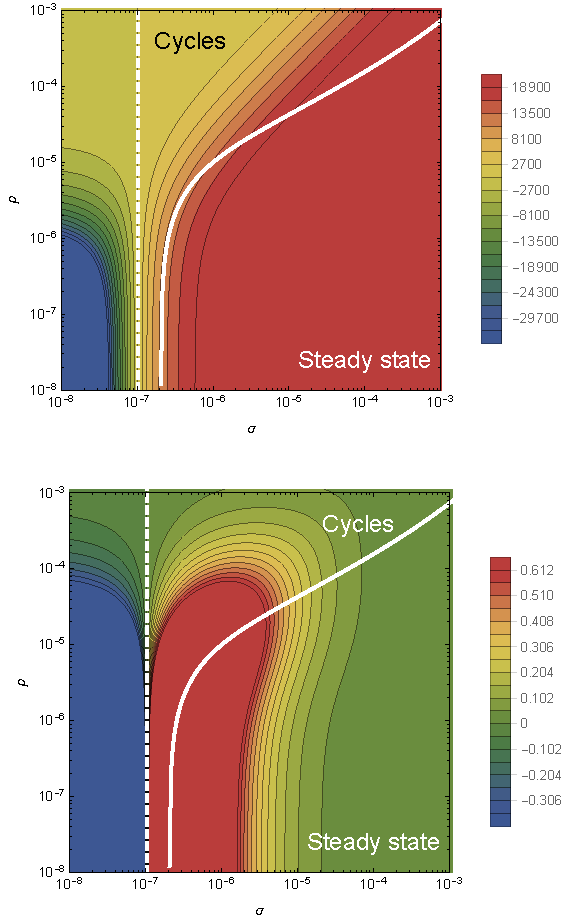
\includegraphics[width=0.5\textwidth]{fig_FixedPoint.pdf}
\caption{ The transcritical (dashed) and Hopf bifurcation (solid) as a
  function of the starvation rate $\sigma$ and recovery rate $\rho$ for a 100g consumer.  These
  bifurcation conditions separate parameter space into unphysical, cyclic,
  and steady state dynamic regimes.  The colors show the steady
  state densities for (\emph{A}) the resource $R^*$ and the (\emph{B}) energetically
  replete consumers $F^*$, (warmer colors denote higher densities).  Steady
  state densities for the energetically deficient consumers $H^*$ (not shown)
  scale with those for $F^*$.  }
\label{fig:fp}
\end{figure*}


\begin{figure*}
\centering
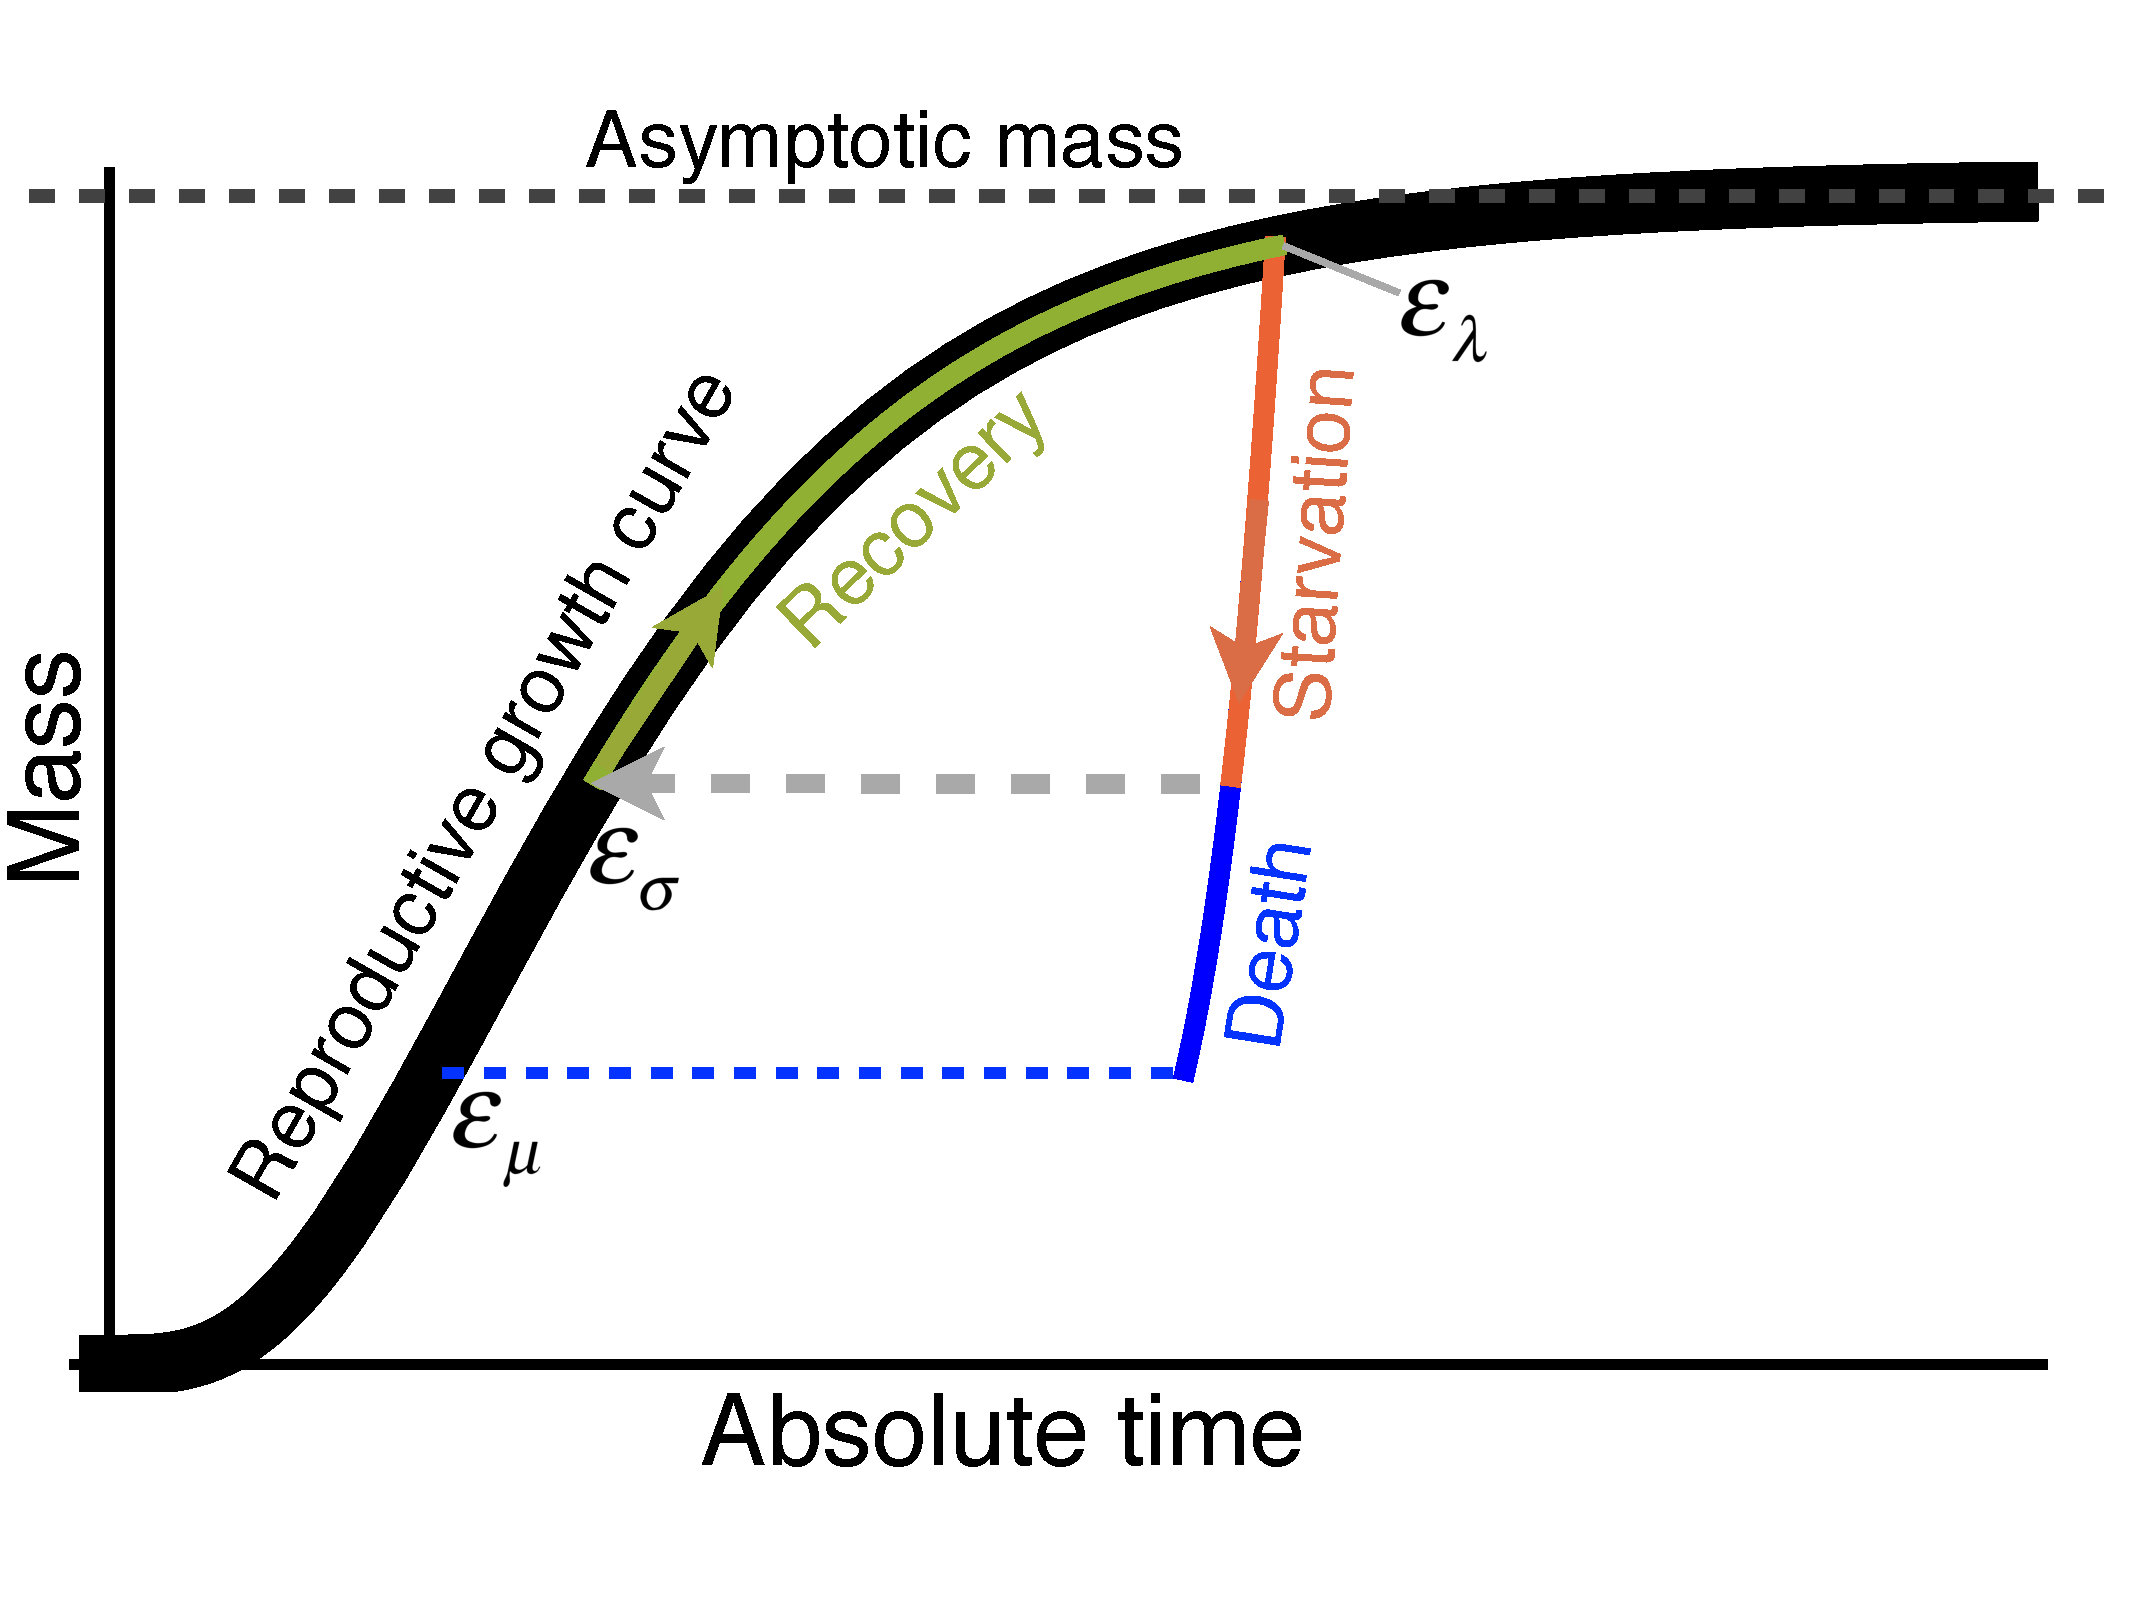
\includegraphics[width=0.5\textwidth]{Growth-trajectory-diagram.pdf}
\caption{ The growth trajectory over absolute time of an individual organism
  as a function of body mass.  Initial growth follows the black trajectory to
  an energetically replete reproductive adult mass $m=\epsilon_\lambda M$ which we assume is 95\% asymptotic mass $M$.  Starvation follows the red
  trajectory to $m = \epsilon_\sigma \epsilon_\lambda  M$. Recovery follows the
  green curve to the replete adult mass, where this trajectory differs from the original growth because only fat is being regrown which requires different energetics and a longer time to reach $\epsilon_\lambda M$. Alternatively, death from starvation follows the blue trajectory to $m=\epsilon_\mu \epsilon_\lambda  M$.}
\label{fig:growth}
\end{figure*}

\begin{figure*}
\centering
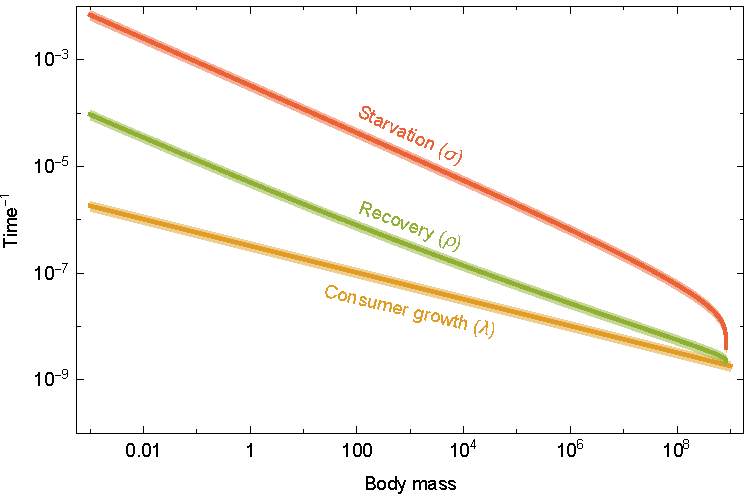
\includegraphics[width=0.5\textwidth]{fig_Rates.pdf}
\caption{
Allometrically constrained starvation rate $\sigma=1/t_{\sigma}$ (red), mortality $\mu=1/t_{\mu}$ (red) and recovery rate $\rho=1/t_{\rho}$ (green) relative to the reproductive rate $\lambda=1/t_{\lambda}$ (black) as a function of body mass (see Equations \ref{t1}, \ref{rhotimescale}, \ref{eq:sigma}, and \ref{mutimescale}).
The rate of starvation is greater than the rate of reproduction for all realized terrestrial endotherm body sizes.
Mean values $\pm 25\%$ variation are shown by the shaded region for each rate.
}
\label{fig:gvs}
\end{figure*}


\begin{figure*}
\centering
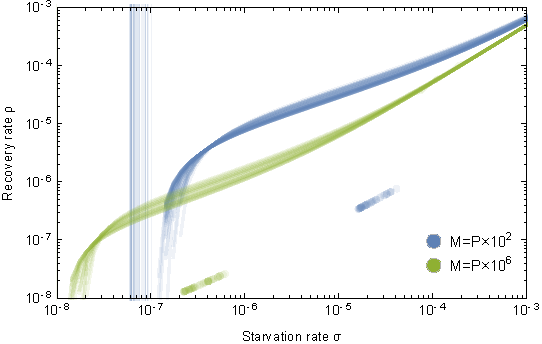
\includegraphics[width=0.5\textwidth]{fig_DataHopf.pdf}
\caption{ Transcritical (vertical lines) and Hopf bifurcations (curves) for
  allometrically determined starvation $\sigma$ and recovery $\rho$ rates as
  a function of different mammalian body sizes: $M=P\times10^2$g (blue) and
  $M=P\times10^6$g (green), where $P$ is a random uniform variable in $[1,9]$.
  Points denote realized values of $\sigma$ and $\rho$ given the drawn values for $M$.
  }
\label{fig:hopf}
\end{figure*}

\begin{figure*}
\centering
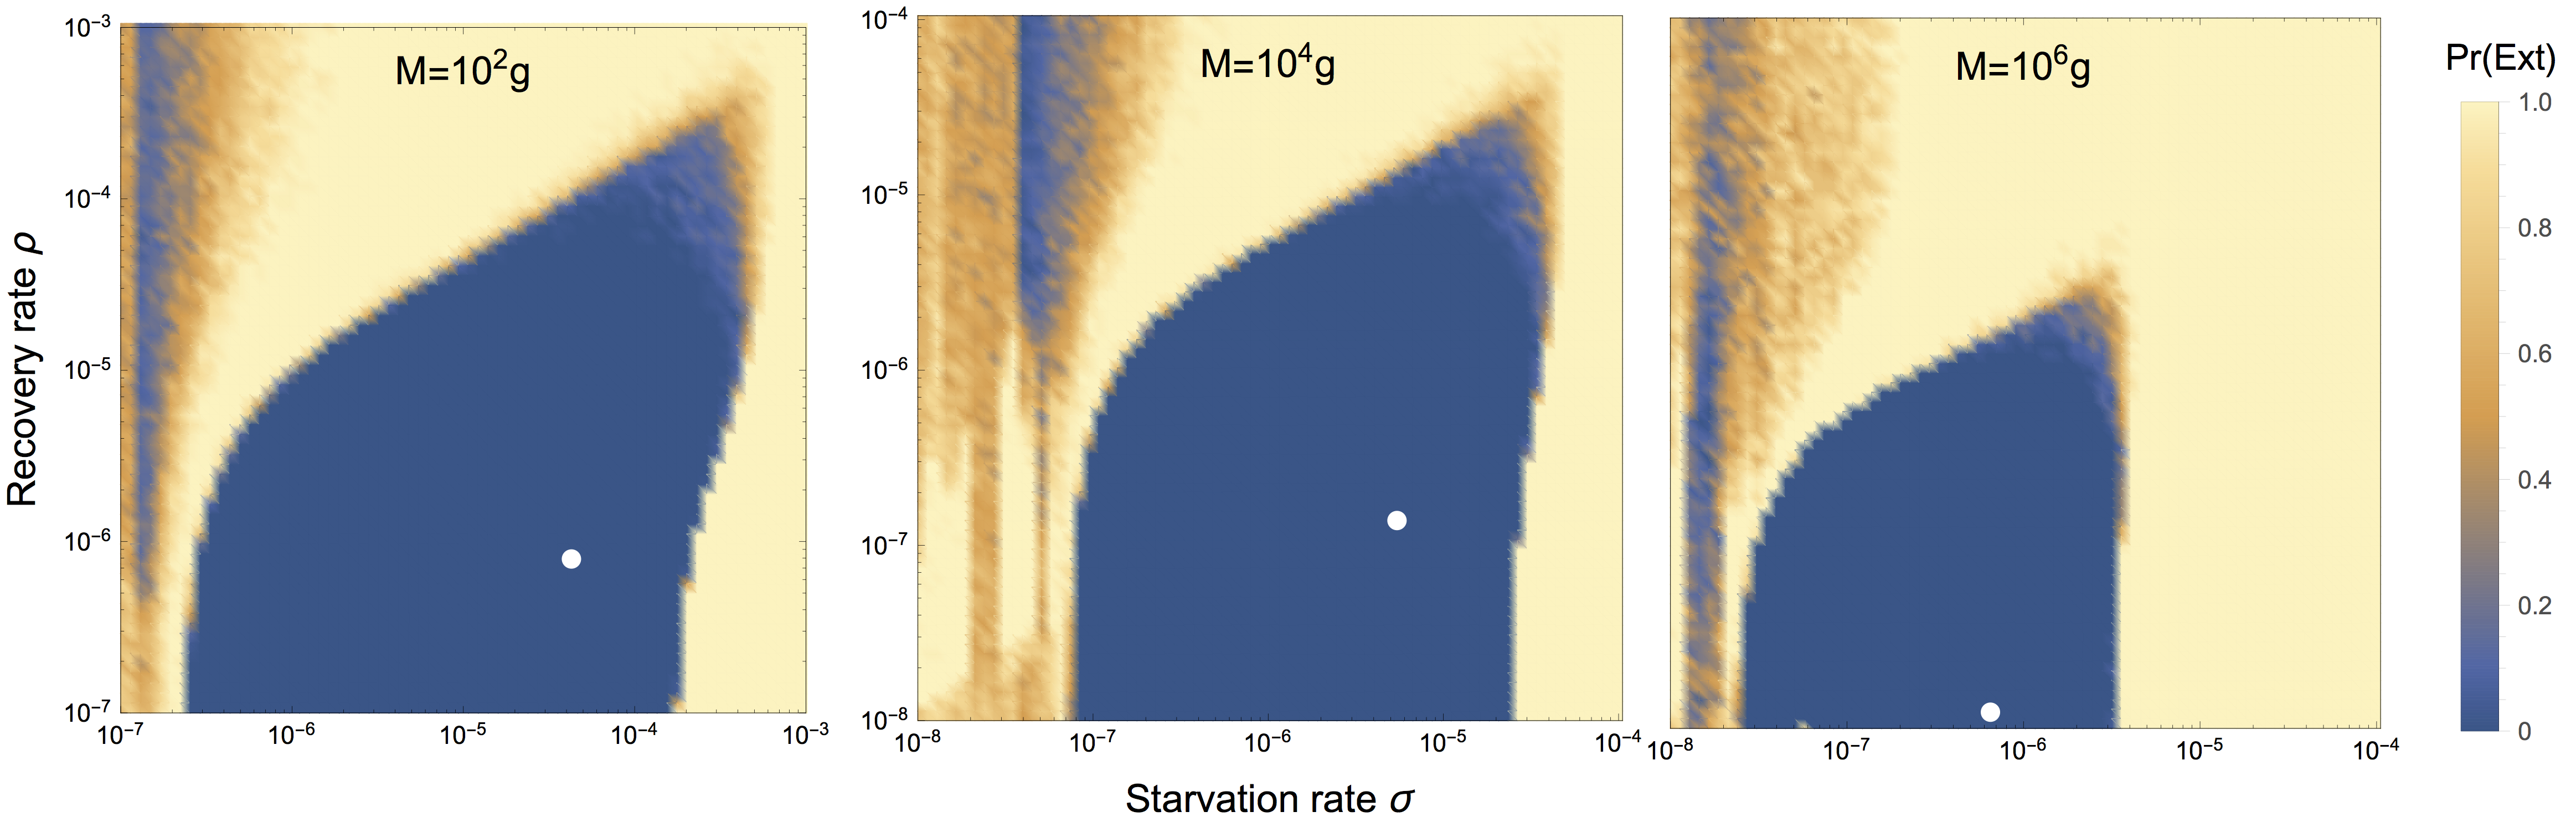
\includegraphics[width=1\textwidth]{fig_ExtinctionAllometricComb3.png}
\caption{ Probability of extinction for a consumer with (from left to right) $M=10^2,~10^4,~10^6$g as a function of the starvation rate $\sigma$ and recovery rate $\rho$, where the initial density is given as $(XF^*,XH^*,R^*)$, where $X$ is a random uniform variable in $[0,2]$. Note the change in scale for $M=10^4,~10^6$g.  Extinction is defined as the population trajectory falling below $0.2\times$ the allometrically constrained steady state. The white points denote the allometrically constrained starvation and recovery rate.}
\label{fig:ext}
\end{figure*}

\begin{figure*}
\centering
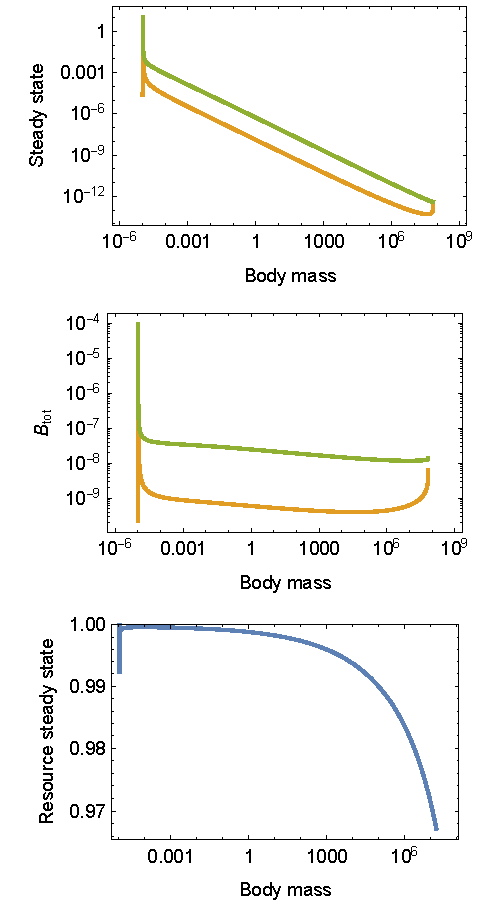
\includegraphics[width=0.45\textwidth]{fig_FPAllometric.pdf}
\caption{ (\emph{A}) Consumer steady states $F^*$ (green) and $H^*$ (orange) as a function of
  body mass.
  (\emph{B}) Total energetic use $B_{\rm tot}$ of consumer populations at the steady state as a function of body mass.
  (\emph{C}) Resource steady state $R^*$ as a function of consumer body mass. The data are from Damuth \cite{damuth1987interspecific} and have been converted to total population metabolism using the allometric relationships for metabolic rate (please see SI and Refs. \cite{West:2001bv,hou,moses2008rmo}).}
\label{fig:mass}
\end{figure*}

\begin{figure*}
\centering
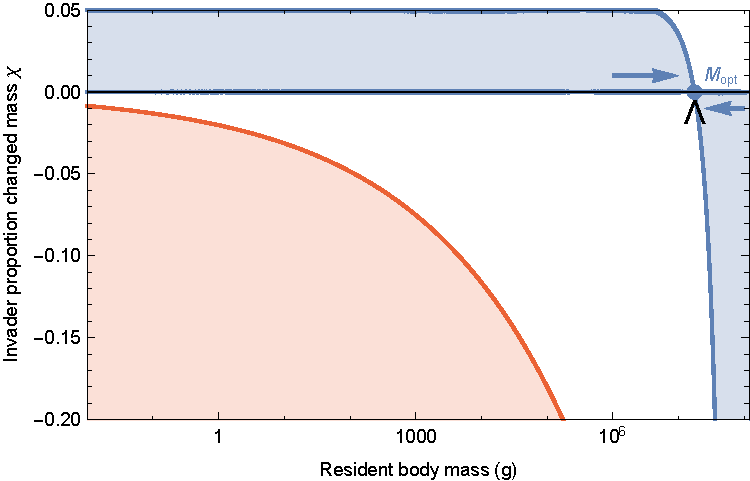
\includegraphics[width=0.75\textwidth]{fig_Invasion.pdf}
\caption{ Invasion feasibility for organisms with a proportional change in
  mass $\chi$ against a population with a resident body mass $M$.  The blue
  region denotes proportions of modified mass $\chi$ resulting in successful invasion.  The
  red region denotes values of $\chi$ that result in a mass that is below the
  starvation threshold and is thus infeasible.
  Arrows point to the predicted optimal mass $M_{\rm opt}=1.75\times 10^7$, which serves as an evolutionary attractor for body mass.
  The black wedge points to the largest body mass known for terrestrial mammals at $7.74\times10^7$g~\cite{Smith:2010p3442}.}
\label{fig:invasion}
\end{figure*}


%
%
%	 \begin{figure}[h]
%		 \centering
%		 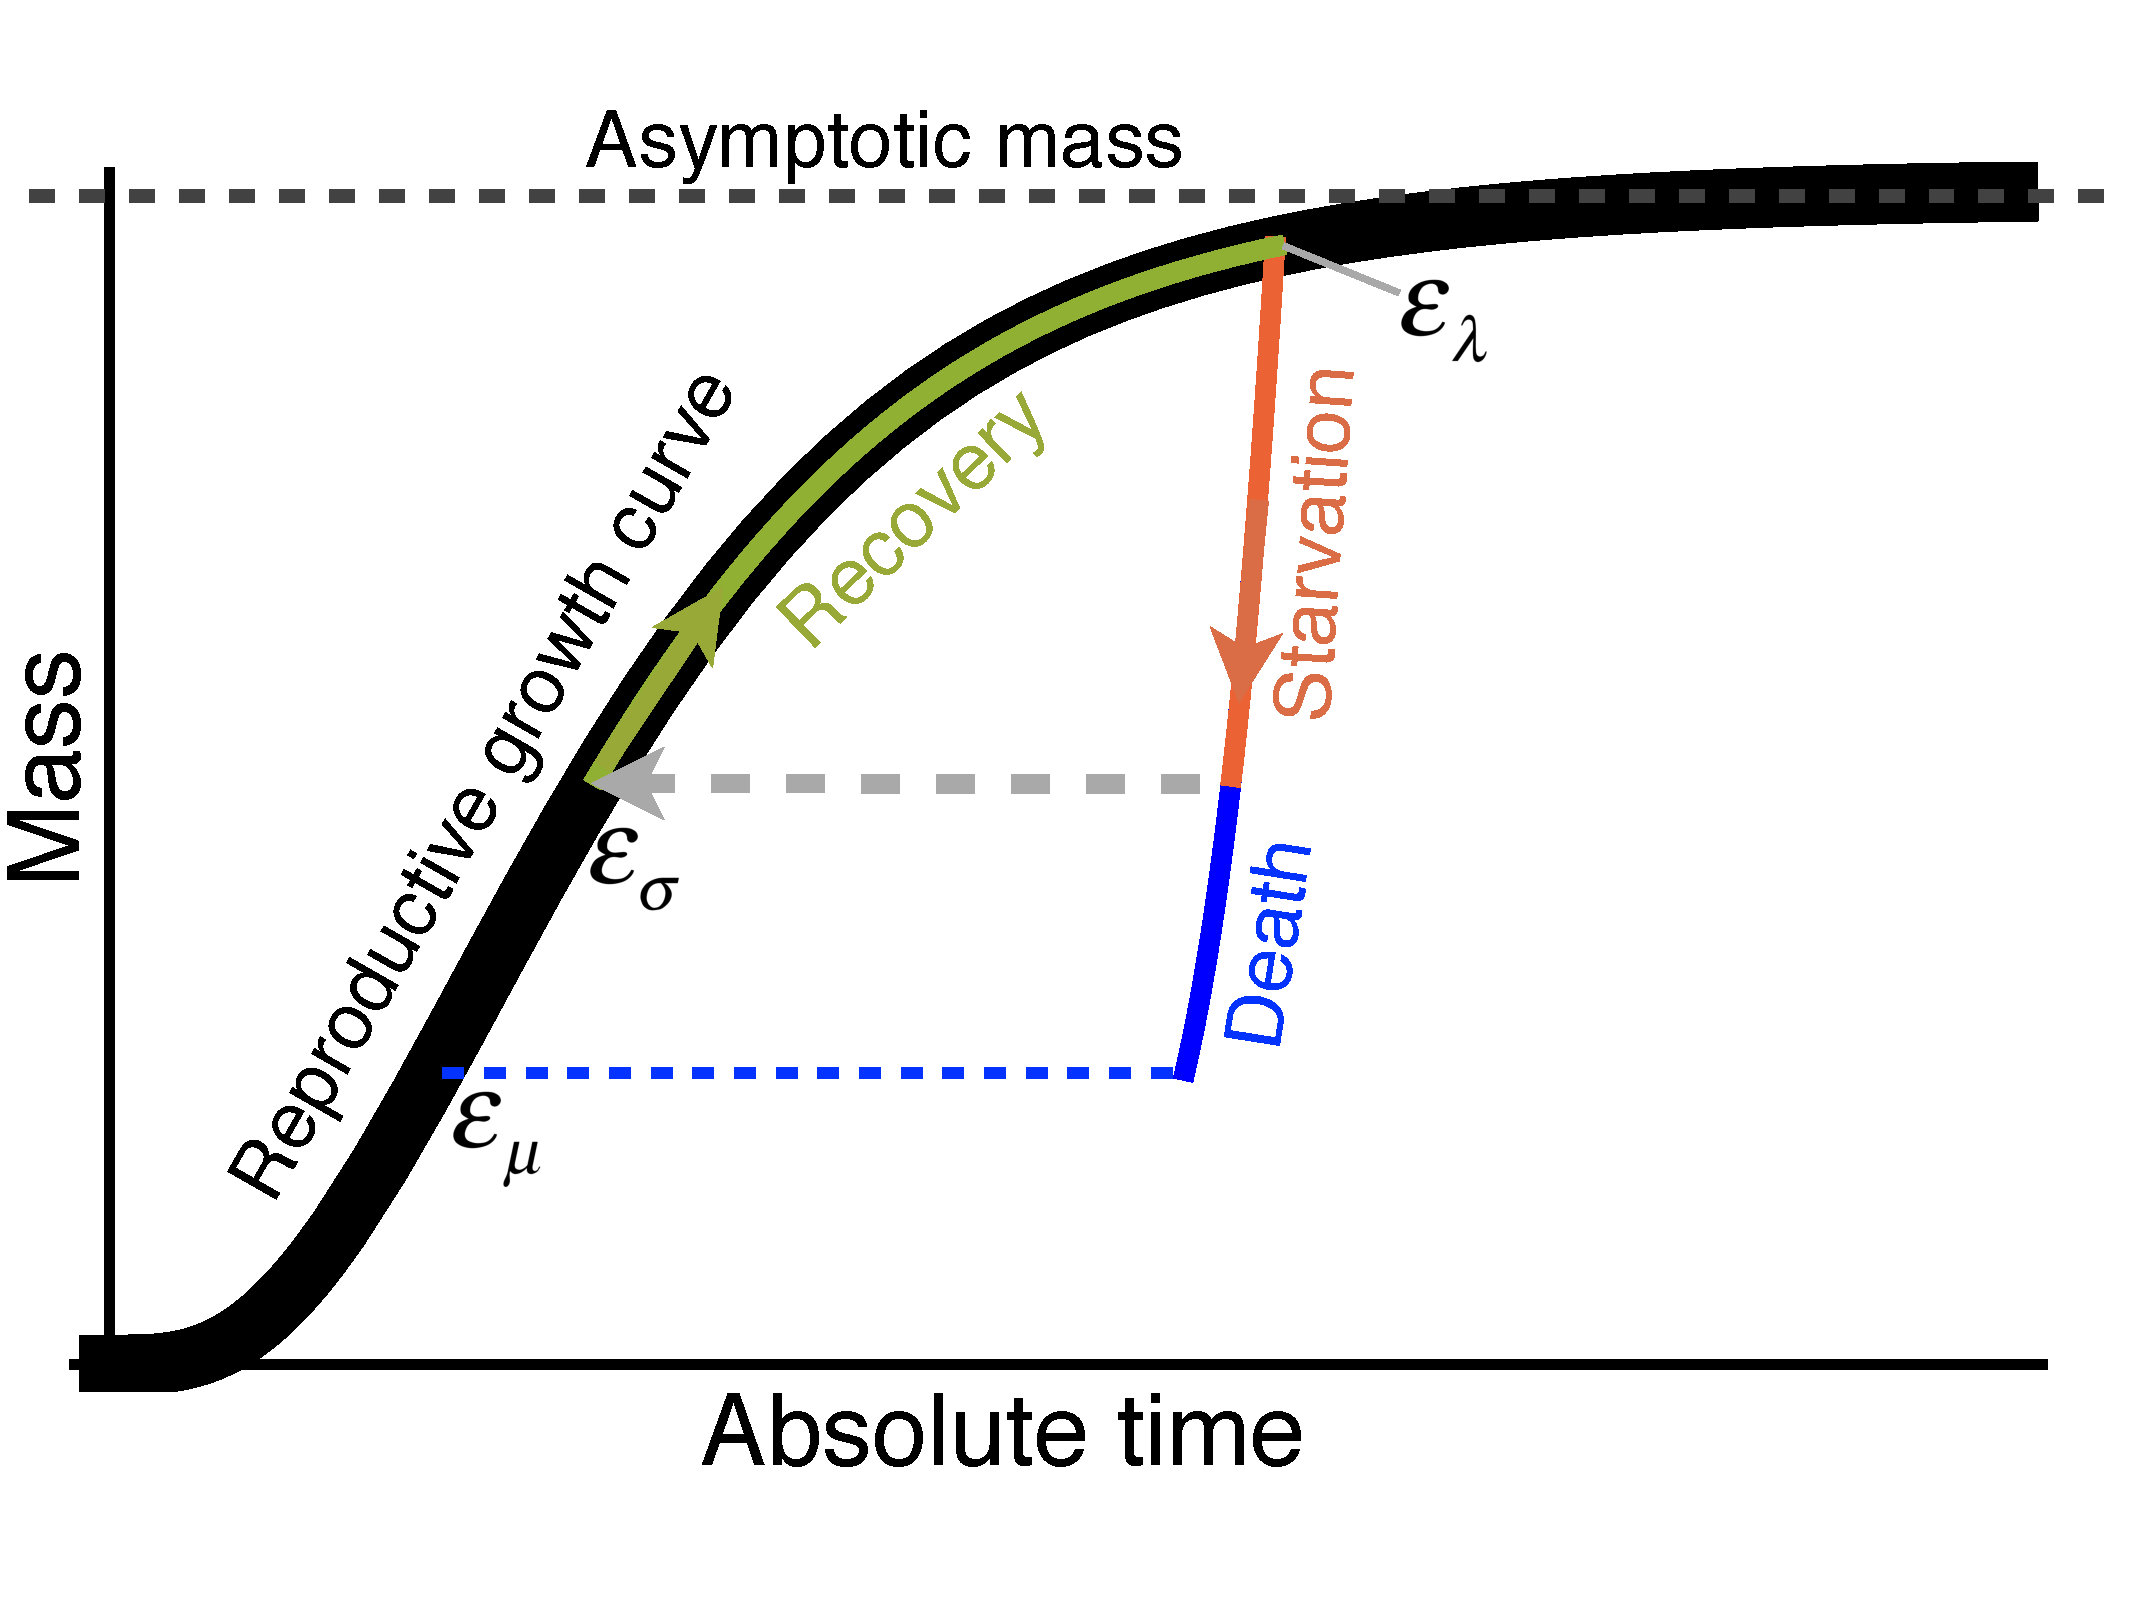
\includegraphics[width=0.5\textwidth]{Growth-trajectory-diagram.pdf}
%		 \caption{
%		 }
%		 \label{growth-diagram}
%	 \end{figure}
%
%	 \begin{figure}[h]
%		 \centering
%		 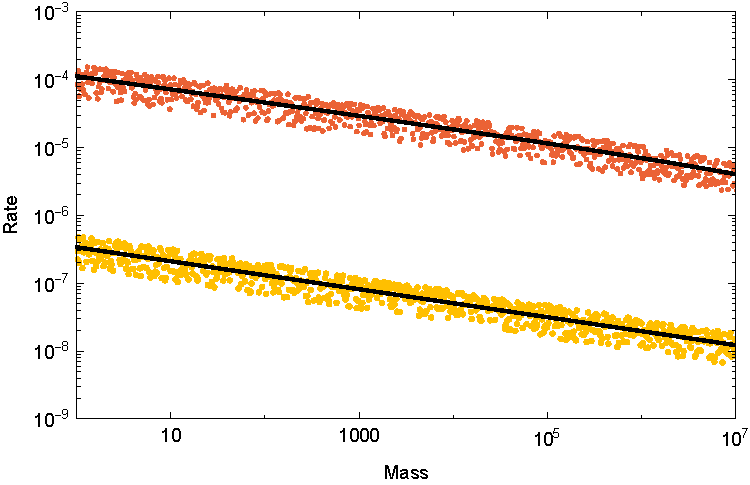
\includegraphics[width=0.25\textwidth]{fig_GvS.pdf}
%		 \caption{
%		 }
%		 \label{GvS}
%	 \end{figure}
%
%
%	\begin{figure}[h]
%	 	\centering
%	 	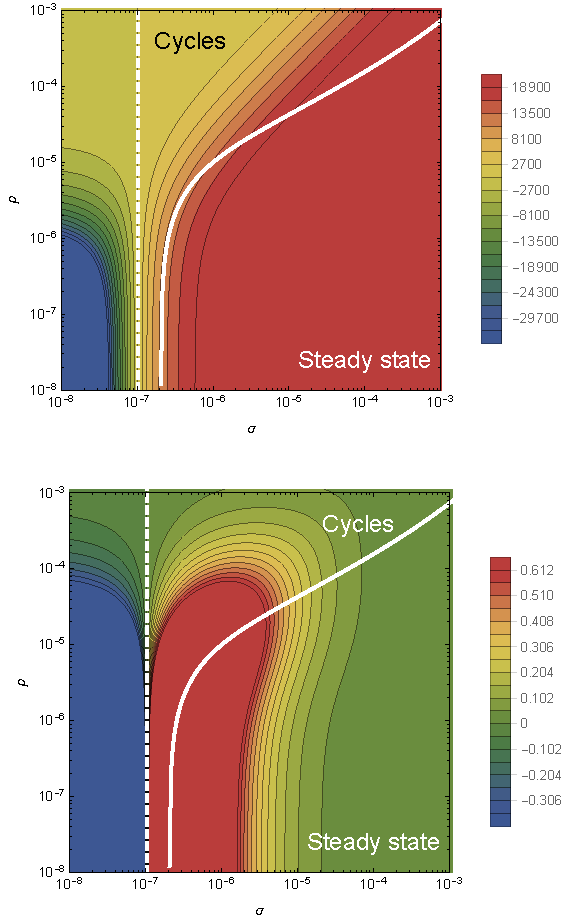
\includegraphics[width=0.25\textwidth]{fig_FixedPoint.pdf}
%	 	\caption{
%	 	}
%		\label{Hopfb}
%	\end{figure}
%
%
%	\begin{figure}[h]
%		\centering
%		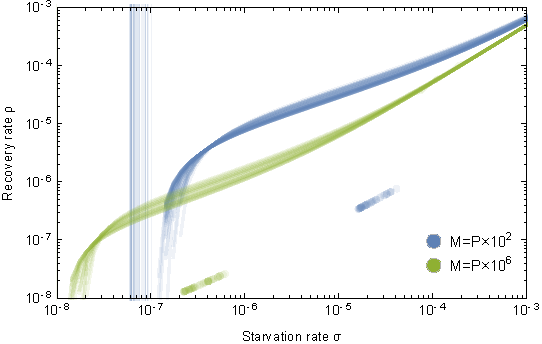
\includegraphics[width=0.8\textwidth]{fig_DataHopf.pdf}
%		\caption{
%		}
%		\label{DataHopf}
%	\end{figure}
%
%
%	\begin{figure}[h]
%		\centering
%	 	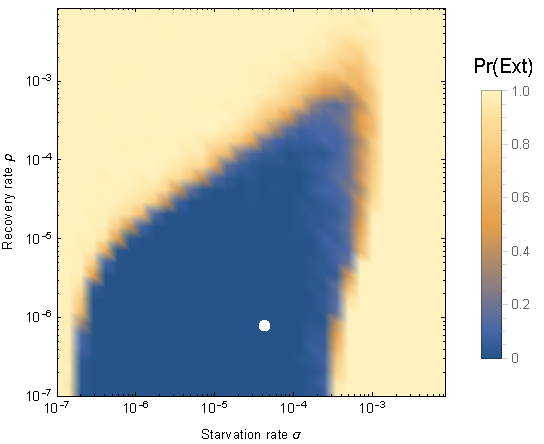
\includegraphics[width=0.8\textwidth]{fig_ExtinctionAllometric.pdf}
%	 	\caption{
%	 	}
%	 	\label{Ext}
%	\end{figure}
%
%	\begin{figure}[h]
%	 	\centering
%	 	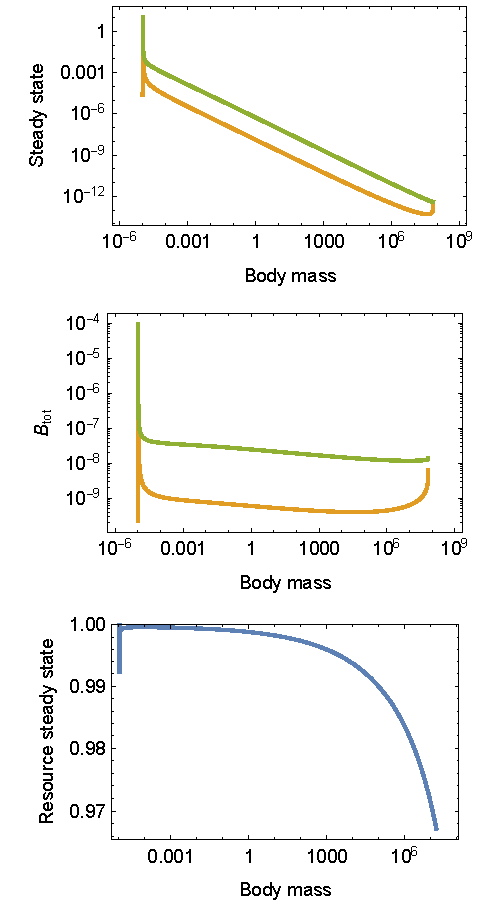
\includegraphics[width=0.5\textwidth]{fig_FPAllometric.pdf}
%	 	\caption{
%	 	}
%	 	\label{Asymp}
%	\end{figure}
%
%\clearpage

%\begin{table}[h]
%\caption{Parameter Values For Various Classes of Organisms}
%\label{param}
%    \begin{center}
%    \small
%     \begin{tabular}{| p{1.2cm}| p{3.2cm} | p{2.6cm} | p{3.2cm} | }
%     \hline
%     & {\bf Mammals} & {\bf Unicellular Eukaryotes} & {\bf Bacteria} \\
%     \hline
%   $\eta$ & $3/4$ & & $1.70$ \\
%   $E_{m}$ & $10695$ (J gram$^{-1}$) & & $10695$ (J gram$^{-1}$) \\
%   $E_{m}^{\prime}$ & $\approx E_{m}$ & & $\approx E_{m}$ \\
%   $B_{0}$ & $0.019$ (W gram$^{-\alpha}$) & & $1.96\times10^{17}$ \\
%   $B_{m}$ & $0.025$ (W gram$^{-1}$)   & & $0.025$ (W gram$^{-1}$)\\
%   $a$ & $1.78\times10^{-6}$ & & $1.83\times10^{13}$ \\
%   $b$ & $2.29\times10^{-6}$ & & $2.29\times10^{-6}$ \\
%   $\eta-1$ & $-0.21$ & & $0.73$ \\
%   $\lambda_{0}$ & $3.39\times10^{-7}$ (s$^{-1}$ gram$^{1-\eta}$) & & $56493$ \\
%   $\gamma$ & $1.19$ & & $0.68$ \\
%   $f_{0}$ & $0.02$ & & $1.30\times10^{-5}$ \\
%   $\zeta$ & $1.01$ & & \\
%   $mm_{0}$ & $0.32$ & & \\
%
%
%   \hline
%    \end{tabular}
%    \end{center}
%   \end{table}



\end{document}
